\chapter{$\Dsplus$ production in p-Pb collisions at $\s$ = 5.02 TeV as a function of multiplicity}
\label{chap:chap6}

In this Chapter the measurement of the ratios of $\Dsplus$-meson yield to that of the 
non-strange $\Dplus$ meson is presented as a function of the primary
charged-particle multiplicity produced in p-Pb collisions at $\sNN=5.02$ TeV and compared to results from 
pp collisions at $\s=7$ TeV~\cite{Acharya:2017jgo} and Pb-Pb interactions at $\sNN=5.02$ TeV~\cite{ALICE-PUBLIC-2017-003}. 
A primary charged particle is a charged particle with mean proper lifetime $\tau$ larger
than 1 cm, which is either produced directly in the interaction or from decay of particles
with $\tau < 1$ cm/$c$.
Primary charged particles are defined as prompt
particles produced in the collisions, including their decay products,
except those from weak decay of strange particles.
In presence of a medium 
composed of deconfined quarks and gluons, a modification of the hadronisation 
mechanisms is expected due to the possible formation of hadrons via
coalescence of charm quarks with other quarks from the 
medium during the deconfined phase or at the phase boundary
~\cite{Greco:2003mm,Greco:2003vf, Andronic:2007zu, He:2012df}. This coalescence mechanism competes with
fragmentation. The enhancement of strange quark abundance in the QGP 
(see Sec.~\ref{subsec:StrangEnhancSPS}) could affect the production of charmed hadrons if 
the dominant mechanism for D-meson formation at low and 
intermediate momenta is in-medium recombination. 
In particular, the relative yield of $\Ds$ 
mesons with respect to non-strange charmed mesons at low $\pt$ is 
predicted to be enhanced in nucleus-nucleus collisions as compared to pp 
interactions~\cite{Andronic2003,RafelskiKuznetsova,HeFriesRapp}.
The measurements of $\Dsplus$/$\Dzero$ and $\Dsplus$/$\Dplus$ ratios in Pb-Pb collisions presented in 
Chapter~\ref{chap:PbPb} indicate higher values in Pb-Pb than in pp collisions, although
the values are compatible within $1\sigma$ of the combined statistical and systematic uncertainties.
Given the observed increase of strange particle production with increasing particle multiplicity
in pp and p-Pb collisions~\cite{Abelev:2013haa,Adam:2015vsf,ALICE:2017jyt}, which reaches
yields compatible with those observed in Pb-Pb collisions at similar multiplicities. The possible 
hadronisation via coalescence could result in an enhancement 
of the relative yield of $\Dsplus$ meson with respect to non-strange
D mesons in high multiplicity p-Pb collisions.


\section{Event selection}
\label{sec:EvSelpPb}
The analysis was performed on the data sample of p-Pb collisions at $\sNN=5.02$ TeV
collected in 2016.
Events were recorded with a minimum-bias (MB) interaction trigger 
that required coincident signals in both scintillator arrays of the V0 detector.
The V0 timing information was used together with that from the ZDCs for offline rejection 
of events produced by the interaction of the beams with residual gas in the vacuum pipe.
The MB trigger was estimated to be sensitive to about 96.4\% of the p-Pb inelastic cross section.
For the data sample analysed here, the probability of event pile-up in the 
same bunch crossing was below 0.5\% per triggered p-Pb event.
The remaining undetected pile-up is negligible in the present analysis.
An algorithm to detect multiple interaction vertices was used to reduce
the pileup contribution. An event was rejected if a second
interaction vertex was found. Only events with a primary vertex reconstructed within $\pm 10$~cm from the 
centre of the detector along the beam line were considered. 
The number of events passing these selection criteria was about $6\times 10^8$.
This number is larger by a factor of $\sim$6 with respect to the number of events analysed with the p-Pb sample collected in 
2013~\cite{Abelev:2014hha,Adam:2016mkz,Adam:2016ich} where, due to the limited statistics, the measurement of $\Ds$ production
in multiplicity classes was not possible. 
The corresponding integrated luminosity of the current sample is 
$L_{\rm int} =N_{\rm MB}/\sigma_{\rm MB}=292 \pm 11~\mu{\rm b}^{-1}$,
where $\sigma_{\rm MB}=2.09$~b is the MB-trigger cross section  
measured via a van der Meer scan, with negligible statistical uncertainty 
and a systematic uncertainty of 3.7\%~\cite{Abelev:2014epa}.
During the p-Pb data taking, the beam energies were 4~TeV for 
protons and 1.58~TeV per nucleon for lead nuclei. 
With this beam configuration, the nucleon-nucleon centre-of-mass system 
moves in rapidity by $\Delta y_{\mathrm{cms}}=0.465$ in the direction 
of the proton beam. The D-meson analyses were performed in 
the laboratory-frame interval $|y_{\mathrm{lab}}|<0.5$, 
which leads to a shifted centre-of-mass rapidity coverage 
of $-0.96 < y_{\mathrm{cms}} < 0.04$.\\


During the p-Pb data taking, two different detector clusters were used to collect data, depending on the 
availability of the SDD detector in the readout. Consequently, the respective reconstructions have different
detector configurations and their $\pt$ resolution may differ. It was verified that the 
width and the position of the D-meson signal peaks were compatible in the two
reconstructions, as a function of $\pt$.The two samples were hence merged and 
used in the analysis in order to maximise the statistics.

\begin{figure}[h]
\centering
 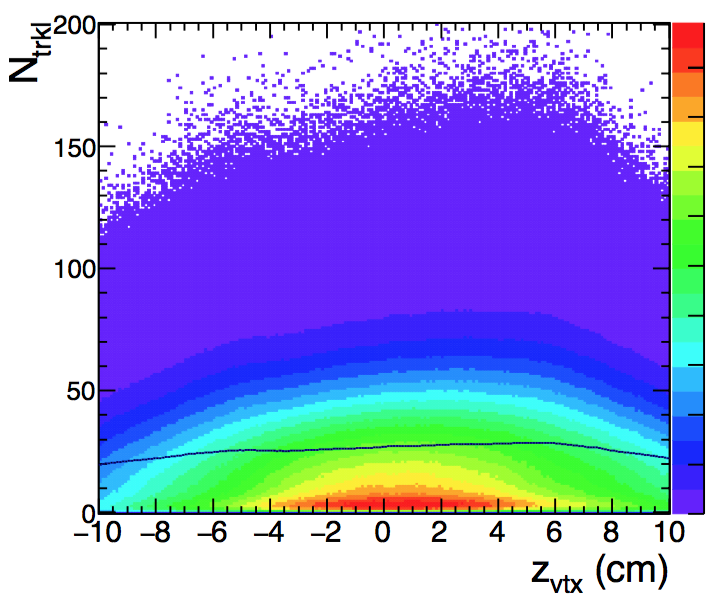
\includegraphics[width=.6\textwidth]{FigCap6/NtrklVsVxtZ_Data.png}
 \caption{$\Ntrkl$ distribution as a function of the $\zVtx$ coordinate.}
 \label{fig:NtrklVsZ2D}
\end{figure}


\section{Equalisation of N$_{\rm tracklets}$ distribution as a function of $z_{\rm vtx}$}
\label{sec:zVxtEq}
The ratios of $\Dsplus$ /$\Dplus$ yields were studied as a 
function the charged-particle multiplicity in different $\pt$ intervals.
The multiplicity estimator used for this analysis was based on the number 
of tracklets reconstructed in the SPD within a 
pseudo-rapidity range of $|\eta| <$ 1. A tracklet in the SPD is obtained by
joining space points on the two SPD layers and it is required to point to 
the reconstructed primary vertex. 
In Fig.~\ref{fig:NtrklVsZ2D}, the distribution of the number of tracklets ($\Ntrkl$) in $|\eta|<1$ as a function
of the $z$ coordinate of the vertex ($\zVtx$) is shown.
 The average number of tracklets $\averNtrkl$ as a function of $\zVtx$ is also shown in the plots.
 The trend of $\averNtrkl$ as a function of $\zVtx$ is related to the SPD geometrical acceptance,
 which does not cover the range $-1 < \eta < 1$ for collisions with $|\zVtx|> 5-6$ cm.
 Lower $\averNtrkl$ values towards $\zVtx \sim 10 $ cm are due to the 
 finite acceptance of the SPD layers. 
The modification of the number of active SPD modules during the data acquisition 
 affects also the number of reconstructed tracklets.
 Therefore, the distribution of $\averNtrkl$ as a function of $\zVtx$ and as a function of the time
 during the data taking needs to be equalised 
in order to consistently define the $\Ntrkl$ intervals in which the analysis is performed.
Otherwise, a given $\Ntrkl$ interval would correspond to different real charged particle
multiplicities, depending on $\zVtx$ or data taking time.
To this purpose, the average profile of $\Ntrkl$ as a function of $\zVtx$ was analysed on a run-by-run basis 
over the full period, to evaluate the stability of $\averNtrkl$ versus $\zVtx$ 
as a function of time. Four bunches of runs were defined corresponding to different SPD
configurations on the A-side of the detector and showing up to $\sim$10\% difference in the $\averNtrkl$ values at positive values 
of $\zVtx$. Fig.~\ref{fig:FourBunches} (left) shows the ratios of the $\Ntrkl$ profiles
of the run groups 1, 2 and 3 to group 4, which is the one with the lowest average tracklet multiplicity.
 The equalisation of $\averNtrkl$ as a function of $\zVtx$ was applied on an 
 event-by-event basis on each of the four groups of runs separately.
The $\averNtrkl$ value that was used as the absolute reference multiplicity 
value was defined as the maximum of $\averNtrkl$ value as a function of $\zVtx$ and time,
resulting $N_{\rm ref} =  29.2$. 
The number $N_{\rm raw}$ of reconstructed tracklets in each event
is corrected by using a Poissonian distribution correction as follows:
\begin{equation} 
\label{eq:NtrklCorr}
N_{\rm trkl}^{\rm corr} = N_{\rm trkl}^{\rm raw} + {\rm Pois}(\Delta N),
\end{equation}
where:
\begin{equation} 
\label{eq:NtrklCorr}
\Delta N = \Big (\frac{N_{\rm ref}}{\langle N(\zVtx) \rangle} -1 \Big ) \cdot N_{\rm trkl}^{\rm raw}.
\end{equation}
 The reference multiplicity value $N_{\rm trkl}^{\rm ref}$ was chosen as the
 maximum value of the $\averNtrkl$ distribution, in order to assure
 that $\Delta N$ follows a Poissonian distribution. 
The average $\averNtrkl$ profiles of the four bunches of runs 
after the $\zVtx$ equalisation are shown in the right panel of 
Fig.~\ref{fig:FourBunches}. They were fitted with a pol1 function in order
to check the flatness of the distribution. The slope of the fit function resulted compatible with zero
validating the efficiency of the correction procedure.

\begin{figure}[h]
\centering
 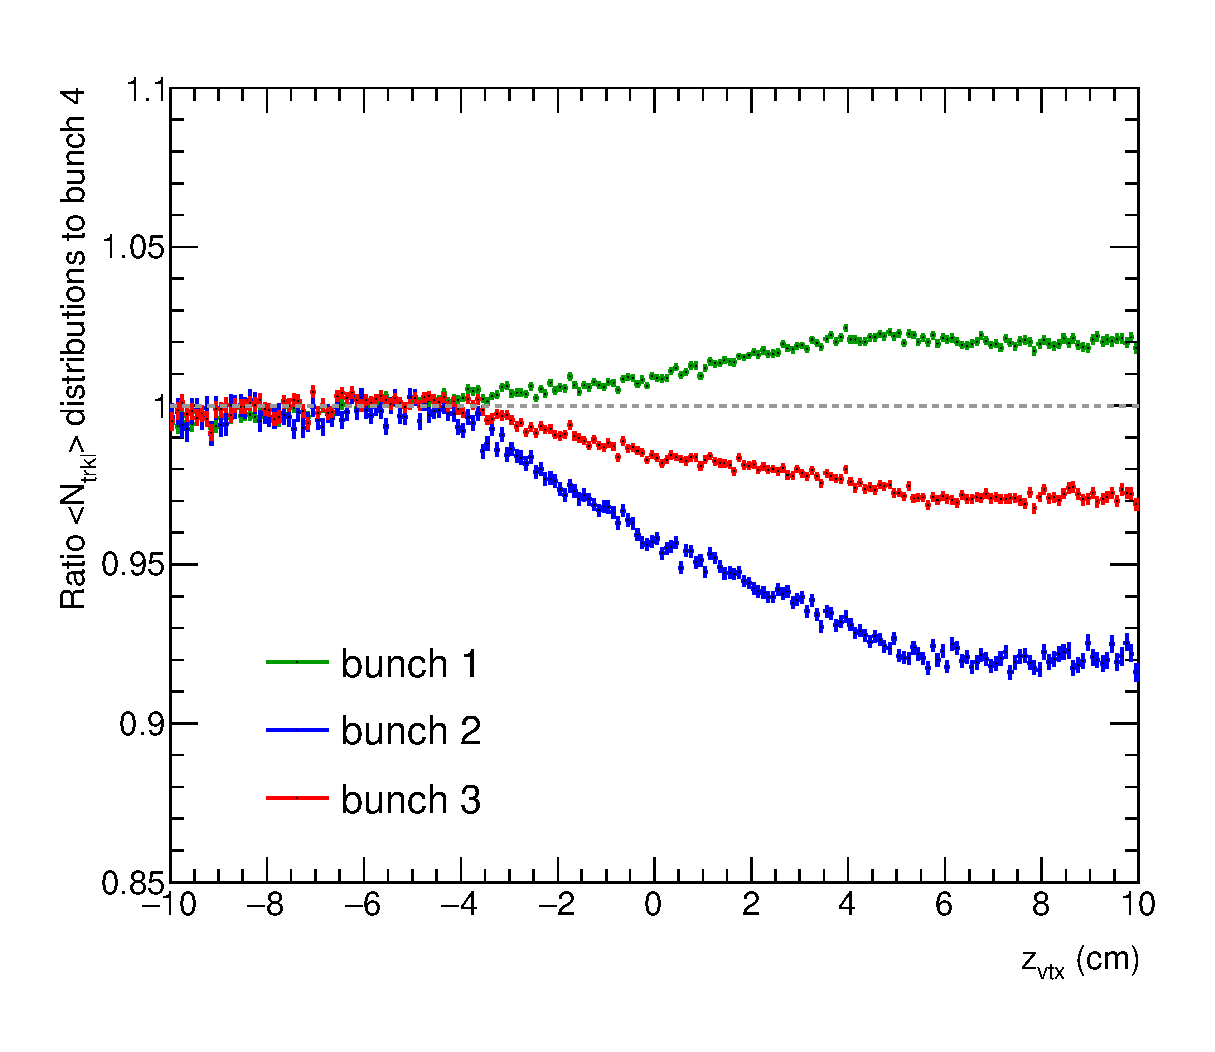
\includegraphics[width=.49\textwidth]{FigCap6/UncorrNtrklProfileDataRatio.eps}
 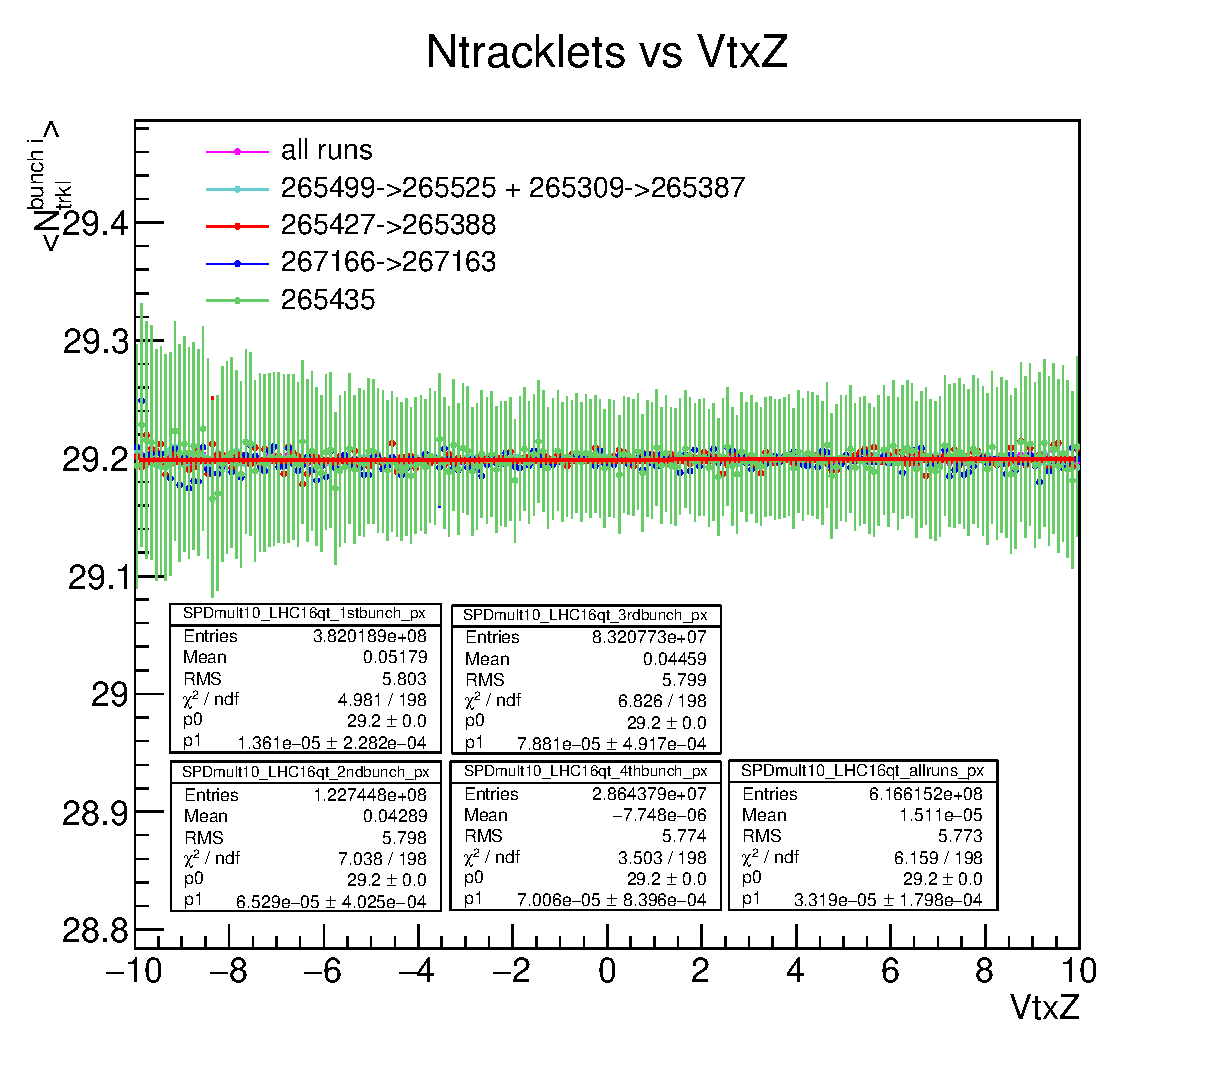
\includegraphics[width=.49\textwidth]{FigCap6/NtrkProfilesDataAfterZVxtEqual.eps}
 \caption{Left: ratio of $\averNtrkl$ distributions of run groups 1, 2 and 3 to group 4 in different colours, as a function of $\zVtx$. Right: $\averNtrkl$ distributions as a function of $\zVtx$ for the four groups of runs in different colours, after equalisation over $\zVtx$.}
 \label{fig:FourBunches}
\end{figure}

\section {Raw-yield extraction}
\label{sec:Rawyields_vs_mult}
The $\Ds$ signal was extracted in five $\pt$ intervals from 2 to 16 $\Gevc$, 
in three different classes of $N_{\rm trkl}^{\rm corr}$: $[1,40)$, $[40,70)$, $[70,200]$ tracklets,
corrected for SPD acceptance effects described in Sec.~\ref{sec:zVxtEq}.
The intervals were chosen in order to have sufficient statistics for the $\Ds$-meson yield extraction.
They contain, in the order, 26.7\%, 45.3\% and 28\% of total number of events.
The $\DstoKKpi$ candidates were built from triplets of tracks as described in Chapter~\ref{chap:pp}
and they were selected by applying cuts on the displaced vertex topology, the
invariant mass of the K$^+$K$^-$ pair and the d$E$/d$x$ and time of flight of the decay tracks.
The $\Ds$ raw yield was extracted via fits to the invariant-mass distributions of candidates passing the
selection criteria described above. The fit function is composed of two Gaussians to model
the $\Ds$ peak and the $\Dplus$ decay contribution in the same channel of $\Dsplus$ (around 1.88 MeV/$c^2$) 
and an exponential function to describe the background.
The cuts were tuned in each $\pt$ interval to have good statistical significance of the extracted yields
and are summarised in Tab.~\ref{tab:cutsDsVsNtrkl}. The same selection criteria
were used in the three multiplicity classes. The particle identification selection is described in Sec.~\ref{Sec:PID}. 
It considers a track to be compatible with the kaon or pion hypothesis if both its d$E$/d$x$ and time of flight 
are within 3$\sigma$ from the expected values. Tracks without a TOF signal 
(mostly at low momentum) are identified using only the TPC information and requiring a 2$\sigma$ 
compatibility with the expected d$E$/d$x$. 
\begin{table}[h!]
\centering
\begin{tabular}{|l|c|c|c|c|c|}
\hline
$\Ds$ selections & \multicolumn{5}{c|}{$\pt$ interval (GeV/$c$)}\\
\cline{2-6}
  & 2--4  & 4--6 & 6--8 & 8--12 & 12--16\\
\hline
Decay length ($\mum$)        & $>$300 & $>$350 & $>$350 & $>$400& $>$400\\
Decay length XY ($\mum$)     & $>$0 & $>$200 & $>$200 & $>$200 & $>$200\\
Norm Decay length XY          & $>$2.0& $>$0.0 & $>$2.0 & $>$2.0 & $>$2.0\\
Cosine pointing              & $>$0.94 & $>$0.95 & $>$0.95 & $>$0.97 & $>$0.97\\
$\sigma_{vertex}$  (cm)          & $<$0.02 & $<$0.03 & $<$0.03 & $<$0.06 & $<$0.06\\
$\Delta M$ (MeV/$c^{2}$) & $<$8.0 & $<$10.0 & $<$4.5 & $<$9.0 & $<$9.0\\
$\cos \theta^*(\pi)$    & $<$1.0 & $<$1.0 & $<$1.0 & $<$0.95 & $<$0.95\\
$|\cos^3 \theta^\prime({\rm K})|$        & $>$0.10 & $>$0.05 & $>$0.05 & $>$0.05 & $>$0.05\\
Norm. IP residual  & $<$2.5 & $<$2.0 & $<$2.0 & $<$2.0  & $<$2.0 \\
\hline
\end{tabular}
\caption{Selection criteria used for $\Ds$ candidates in the five transverse momentum intervals considered for the three $N_{\rm trkl}$ classes.}
\label{tab:cutsDsVsNtrkl}
\end{table}
Fig.~\ref{fig:DsInvMassVsNtrkl_1},~\ref{fig:DsInvMassVsNtrkl_2} and~\ref{fig:DsInvMassVsNtrkl_3} 
show the invariant-mass fits performed in the five $\pt$ intervals, for the three 
multiplicity classes. 
\begin{figure}[htpb]
\centering
 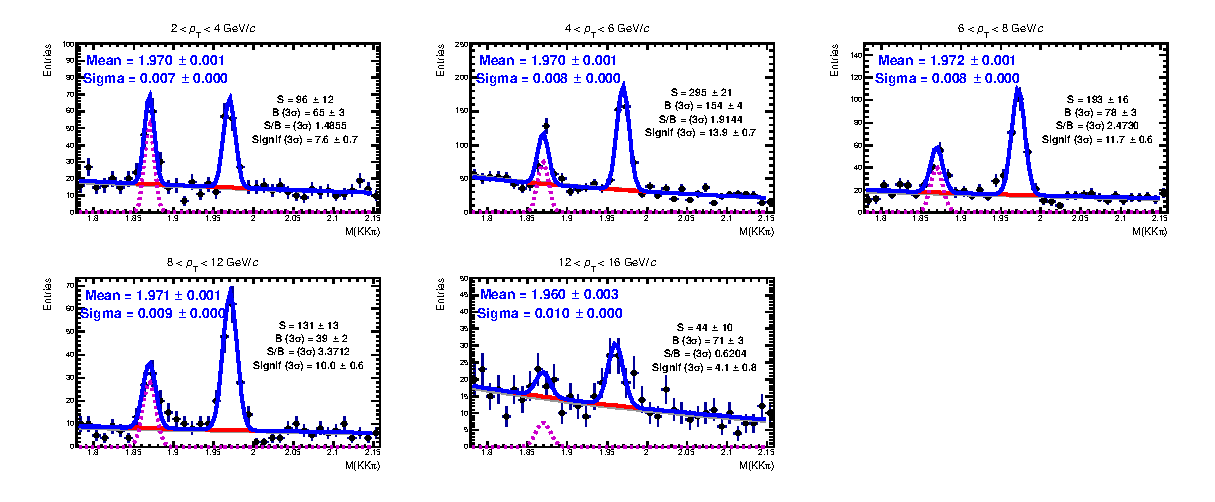
\includegraphics[width=1\textwidth]{FigCap6/DsMass_140Trkl.eps}
  \caption{$\Dsplus$ candidate (and charge conjugates) invariant-mass spectra, in five $\pt$ intervals from $2 < \pt < 16$ $\Gevc$, in the $1 \leq N_{\rm trkl} < 40$ multiplicity interval.}
 \label{fig:DsInvMassVsNtrkl_1}
\end{figure}
\begin{figure}[htpb]
\centering
 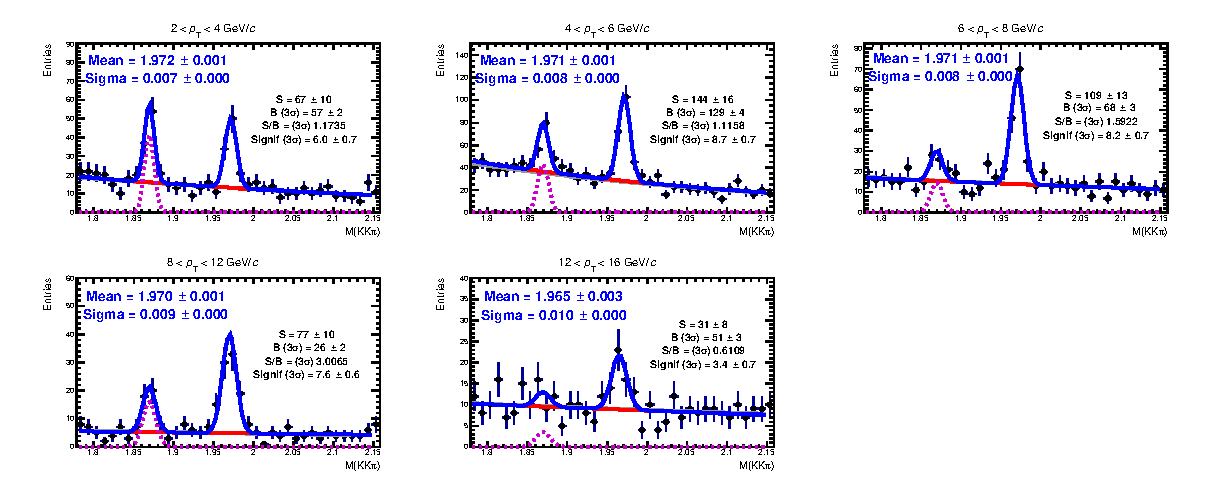
\includegraphics[width=1\textwidth]{FigCap6/DsMass_4070Trkl.eps}
  \caption{$\Dsplus$ candidate (and charge conjugates) invariant-mass spectra, in five $\pt$ intervals from $2 < \pt < 16$ $\Gevc$, in the $40 \leq N_{\rm trkl} < 70$ multiplicity interval.}
 \label{fig:DsInvMassVsNtrkl_2}
\end{figure}
\begin{figure}[htpb]
\centering
 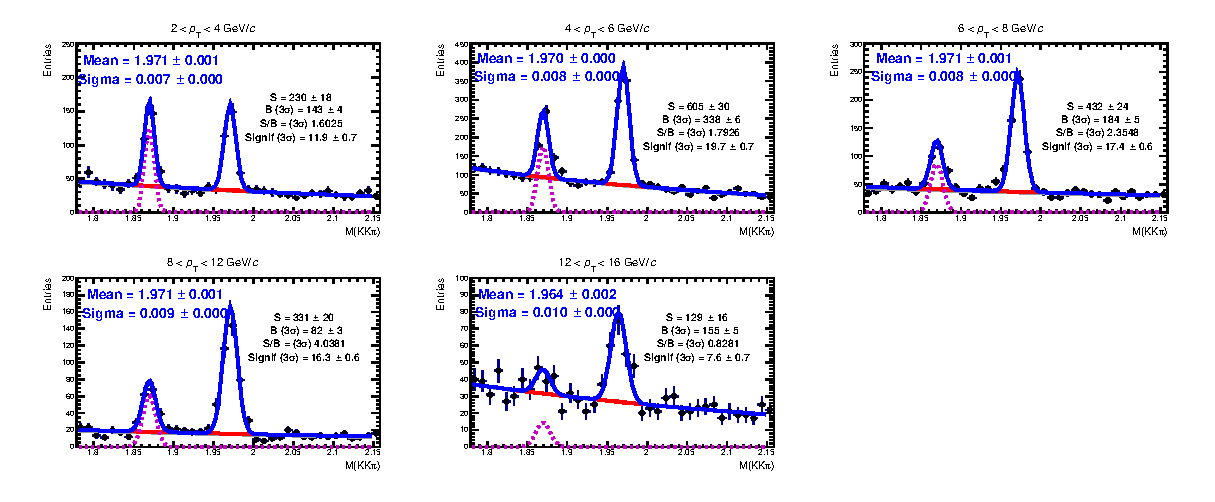
\includegraphics[width=1\textwidth]{FigCap6/DsMass_70200Trkl.eps}
  \caption{$\Dsplus$ candidate (and charge conjugates) invariant-mass spectra, in five $\pt$ intervals from $2 < \pt < 16$ $\Gevc$, in the $70 \leq N_{\rm trkl} \leq 200$ multiplicity interval.}
 \label{fig:DsInvMassVsNtrkl_3}
\end{figure}
To avoid fluctuations, the $\Ds$ peak widths were fixed to the values obtained from the 
multiplicity-integrated sample of simulated $\DstoKKpi$ decays. To this purpose, it was verified that the
width of the $\Ds$ peak in the simulation and in data does not depend on the multiplicity intervals, as it can be seen in Fig.~\ref{fig:MCsigmaCompNtrklBins}, in the left and right panels, respectively. 
In Fig.~\ref{fig:DsFitParamsVsNtrkl} the Gaussian peak positions  
in data for the three intervals of $\Ntrkl$ are compared to the values of the widths extracted from the fit 
on the distribution integrated over multiplicity in data and in the simulation.
\begin{figure}[htpb]
\centering
 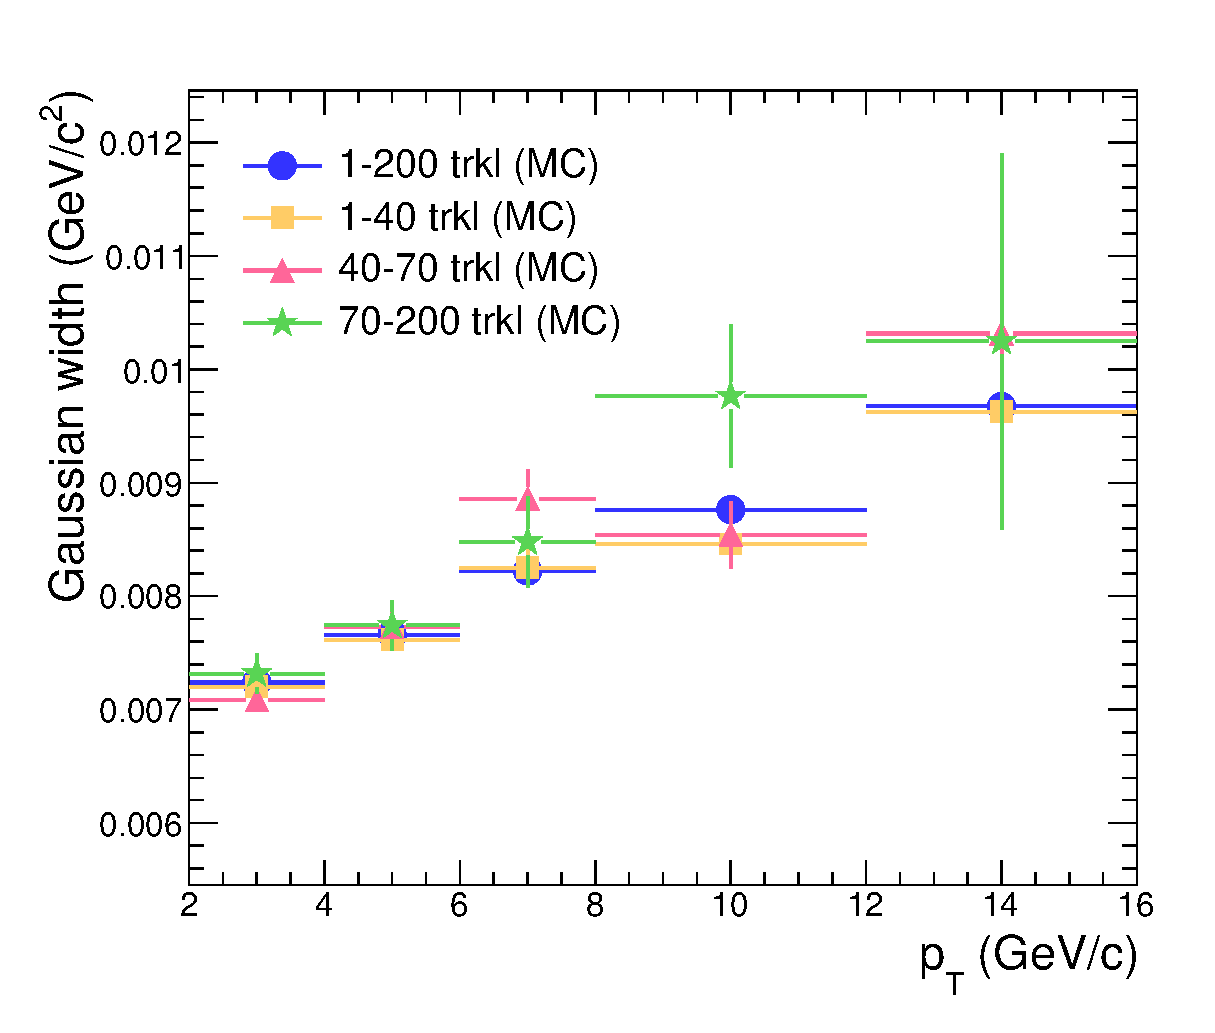
\includegraphics[width=.48\textwidth]{FigCap6/comparisonSigmaDsMCBInsNtrkl.eps}
 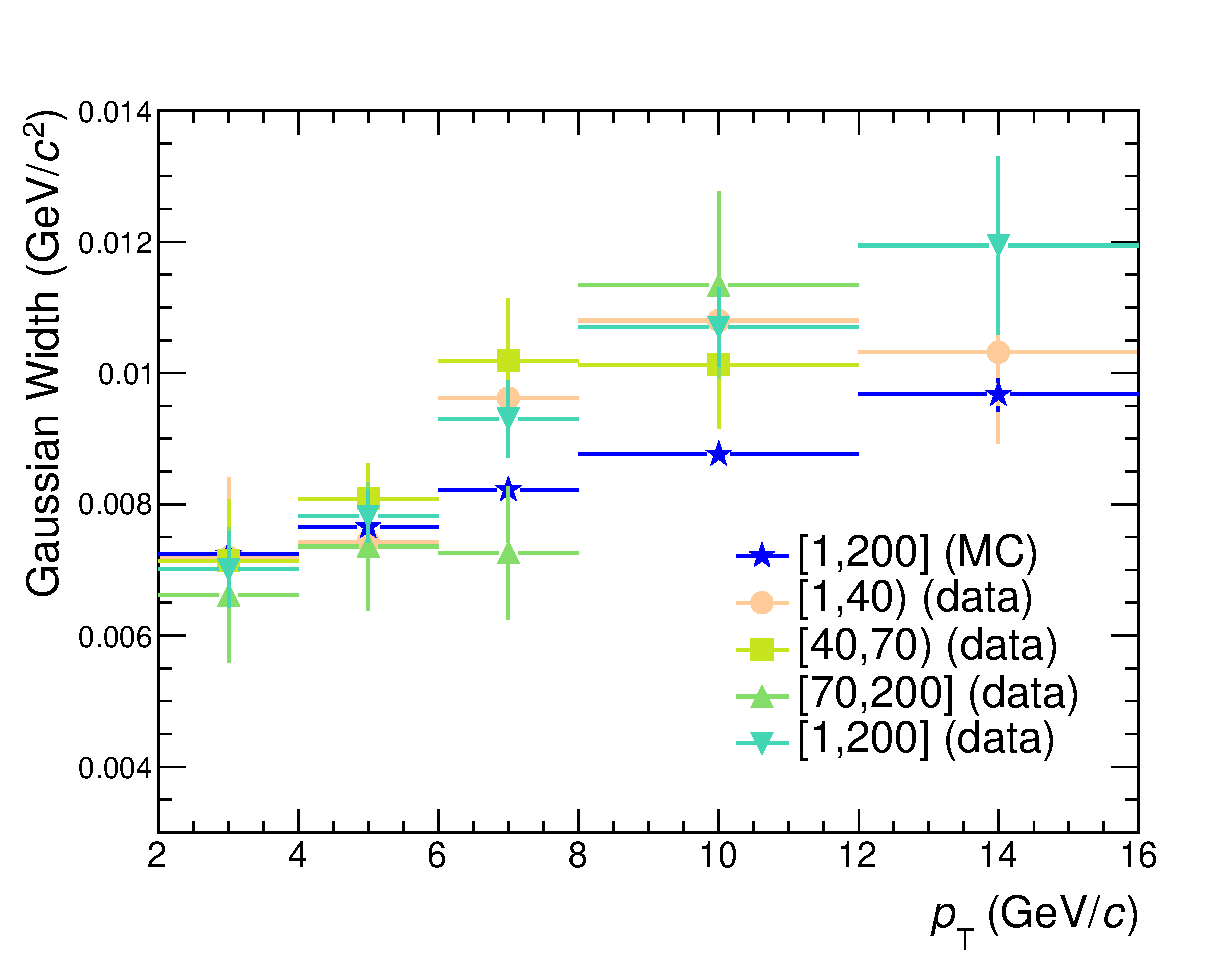
\includegraphics[width=.5\textwidth]{FigCap6/DsSigma_DataMC_AllNtrklInt_Ntrkl.eps}
  \caption{$\Ds$ peak widths as a function of $\pt$, obtained from the fits to the invariant-mass distributions in the three $\Ntrkl$ intervals in simulations (left) and in data (right) compared to the widths extracted from the fit in the sample integrated over multiplicity.}
 \label{fig:MCsigmaCompNtrklBins}
\end{figure}

\begin{figure}[htpb]
\centering
 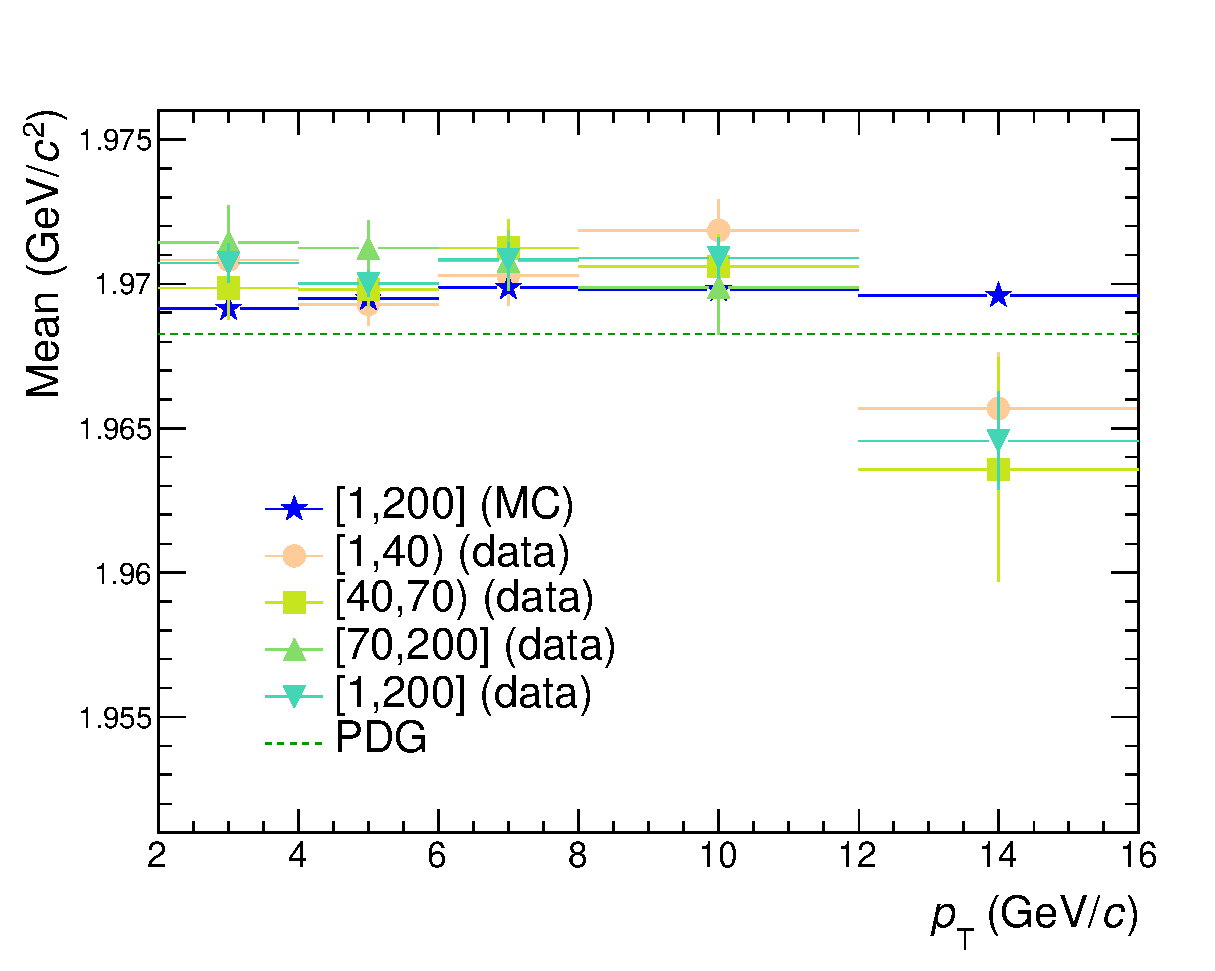
\includegraphics[width=.5\textwidth]{FigCap6/DsMean_DataMC_AllNtrklInt_Ntrkl.eps}
  \caption{$\Ds$ peak position obtained from the fits to the invariant mass distribution in the three intervals of $\Ntrkl$ in data compared to the data and simulations integrated over multiplicity.}
 \label{fig:DsFitParamsVsNtrkl}
\end{figure}

\section{Corrections}
\label{sec:Corrections}
The $\Dsplus$/$\Dplus$ ratios in the multiplicity class $i$ and the $\pt$ interval $j$ were calculated
as:
\begin{equation} 
\label{eq:NtrklCorr}
 \frac{({\rm d}^2N_{\Dsplus}/{\rm d}\pt {\rm d}y)}{({\rm d}^2N_{\Dplus}/{\rm d}\pt {\rm d}y)} \Big |_i = \frac{Y^{i, j}_{\Dsplus}  f^{i, j}_{\rm prompt, \Dsplus} / ({\rm Acc} \times \epsilon)^{i, j}_{\rm prompt \Dsplus}}{Y^{i, j}_{\Dplus}  f^{i, j}_{\rm prompt, \Dplus} / ({\rm Acc} \times \epsilon)^{i, j}_{\rm prompt \Dplus}} \cdot \frac{\rm BR(\DstoKKpi)}{\rm BR(\DplustoKpipi)},
\end{equation}
where $Y^{i, j}_{\rm D}$ is the extracted yield of $\Dsplus$ and $\Dplus$, which is corrected for the prompt fraction
$f^{i, j}_{\rm prompt}$, for the acceptance-times-efficiency term $({\rm Acc} \times \epsilon)^{i, j}$ and for
the branching ratio BR of the decay channel, which is different for $\Dsplus$ and $\Dplus$.\\



The acceptance-times-efficiency term was obtained via Monte Carlo simulations
using PYTHIA v6.4.21~\cite{Sjostrand:2006za} with Perugia-2011 tuning as event generator.  
A HIJING~\cite{Wang:1991hta} p-Pb event is added as underlying event to the PYTHIA
one in a fraction of events corresponding to the probability of having $N_{\rm coll}>1$ in the
Glauber MC simulations of p-Pb collisions. 
Particles were transported through the detectors using the GEANT3 package~\cite{Brun:1994aa}.
Fig.~\ref{fig:NtrklDataMC} (left) shows the distributions of the number of SPD tracklets $\Ntrkl$ in $|\eta|<1$ in data and simulation.
The events selected to fill the distributions were required to have at least a $\DtoKpi$ meson candidate 
passing the selection criteria, with the invariant mass compatible within 3$\sigma$ to the $\Dzero$ mass from PDG 
($\sigma$ being the width of $\DtoKpi$ invariant-mass peak).
The choice of $\Dzero$ meson was made in order to study the multiplicity distribution
of events with charm production which differ from that of minimum bias events.
Measurements in pp collisions~\cite{AguilarBenitez:1988js} show that the events with charm production
have on average higher multiplicity than minimum-bias collisions.
In particular, among the different D-meson species, the $\DtoKpi$ decays
were used in this study because of their large abundance and high signal-to-background ratio.
The distributions in Fig.~\ref{fig:NtrklDataMC} (left) are shown before the correction for the $\zVtx$ equalisation. 
It is evident that the $\Ntrkl$ distributions in data and MC are different.
For this reason, since the selection efficiency depends on multiplicity, the calculation
of $({\rm Acc} \times \epsilon)$ from the simulation was done with 
with data-driven multiplicity weights. These multiplicity weights were extracted
separately for each of the four groups of runs discussed in Sec.~\ref{sec:zVxtEq},
corresponding to different SPD configurations.
The weights were defined as the ratios of the multiplicity distribution in data and in 
the simulations, as their distributions as a function of the $\Ntrkl$ multiplicity are shown in Fig.~	\ref{fig:NtrklDataMC} (right), in 
different colours for the fours groups of runs. The ratios of the weights from the four groups of runs to the ones integrated over
all runs is shown in Fig.~\ref{fig:RatioNtrklMC}.
Furthermore, the simulated $\Ntrkl$ distribution does not reach the highest 
$\Ntrkl$ values observed in data. However, it was verified 
that the selection efficiency of $\Ds$ mesons does not depend on
the tracklet multiplicity for $\Ntrkl > 20$, as it is shown in Fig.~\ref{fig:DsEffVsMult} (left). Hence, the different
maximum $\Ntrkl$ values in data and MC does not introduce a bias.
The efficiencies were re-weighted separately for each of the three intervals of tracklets
in which the analysis was performed, using the procedure discussed above and considering
the respective $N_{\rm trkl}^{\rm corr}$ distributions in data to calculate the weights.
The re-weighted acceptance-times-efficiency values for the three $\Ntrkl$ classes are presented in 
the right panel of Fig.~\ref{fig:DsEffVsMult} as a function of $\Ntrkl$, for the five analysed $\pt$ intervals
in different colours. As shown in this figure, the efficiency is almost flat 
as a function of the event multiplicity.\\


\begin{figure}[h]
\centering
 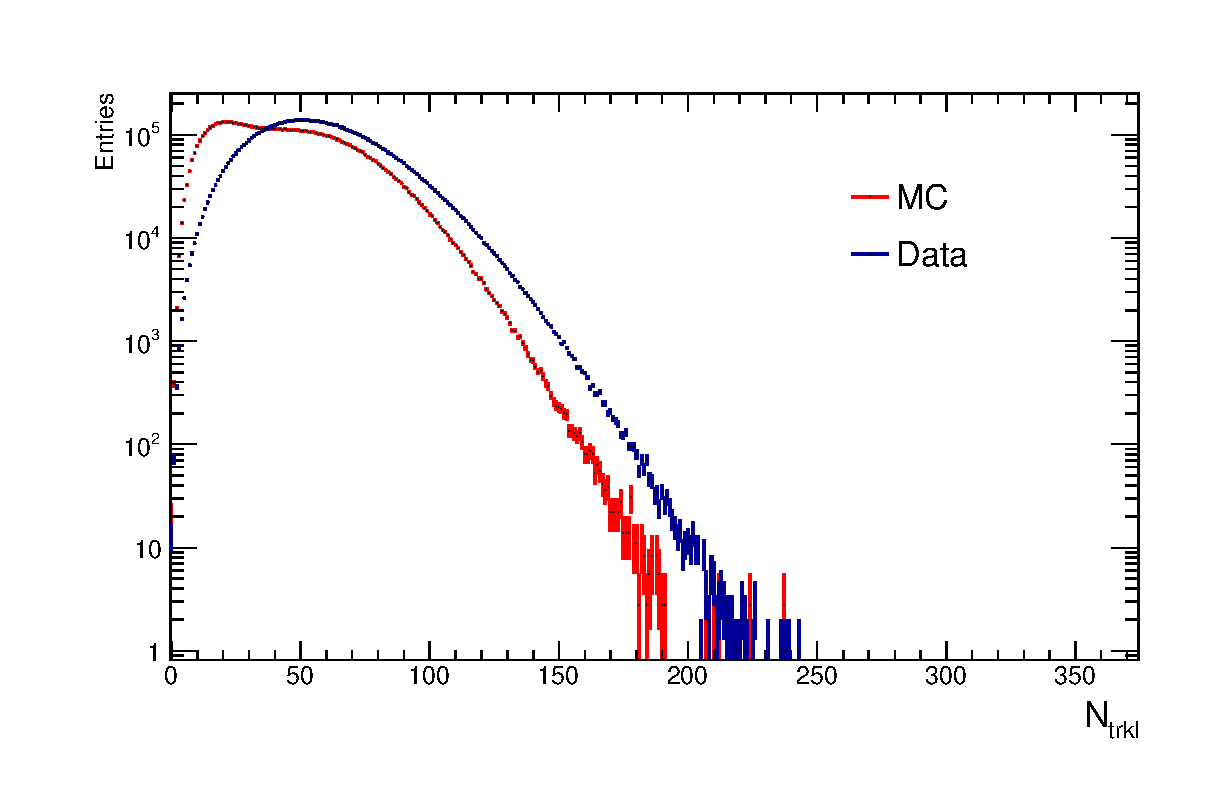
\includegraphics[width=.49\textwidth]{FigCap6/NtrkDistrDDataMC.eps}
 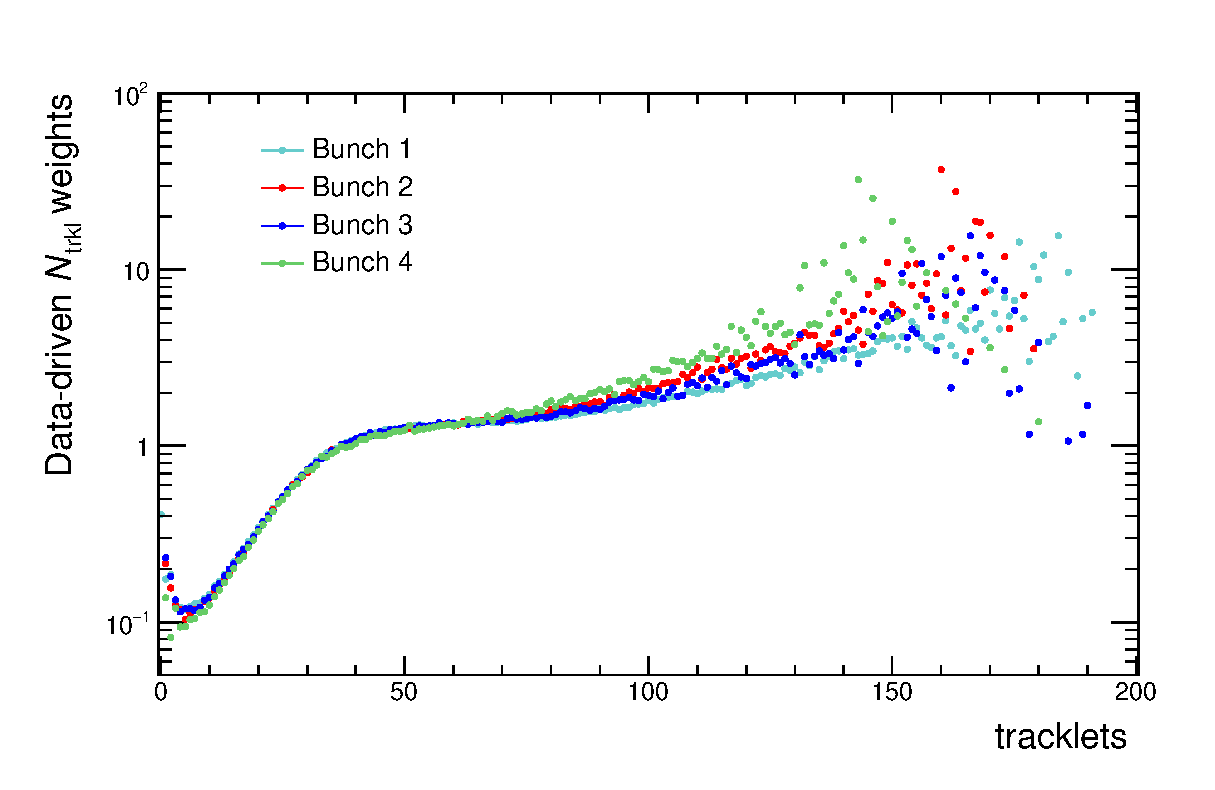
\includegraphics[width=.49\textwidth]{FigCap6/NtrklWeightsMC_4bunches.eps}
 \caption{Left: tracklets distribution in data and in MC in different colours. Right: data-driven weights used to correct the efficiencies as a function of the tracklet multiplicity, for the four groups of runs in different colours.}
 \label{fig:NtrklDataMC}
\end{figure}

\begin{figure}[h]
\centering
 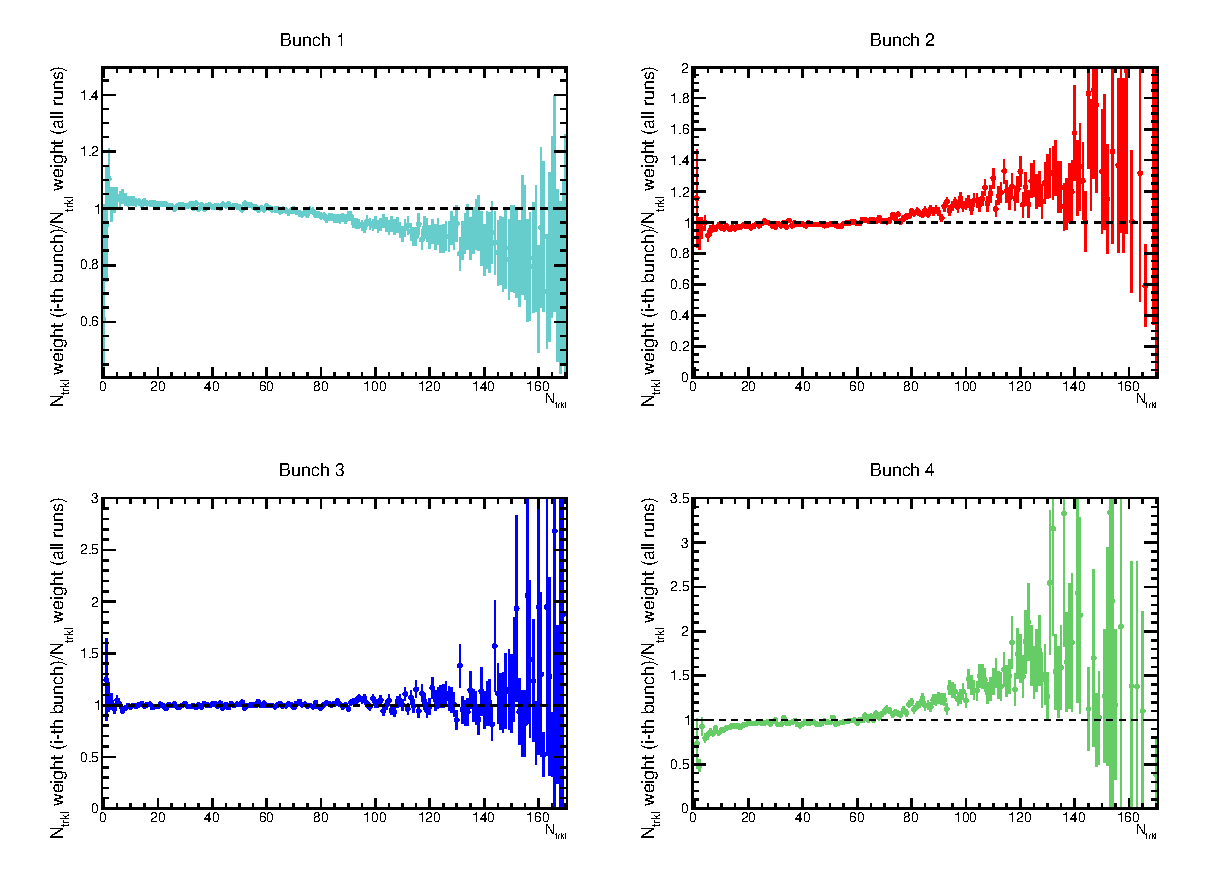
\includegraphics[width=.9\textwidth]{FigCap6/NtrkDistrMC_17d2a_EvWithD_zVxtUnCorr_896_897.eps}
 \caption{Ratios of multiplicity weights for each of the four groups of runs to the weights computed for the full sample.}
 \label{fig:RatioNtrklMC}
\end{figure}

\begin{figure}[h]
\centering
 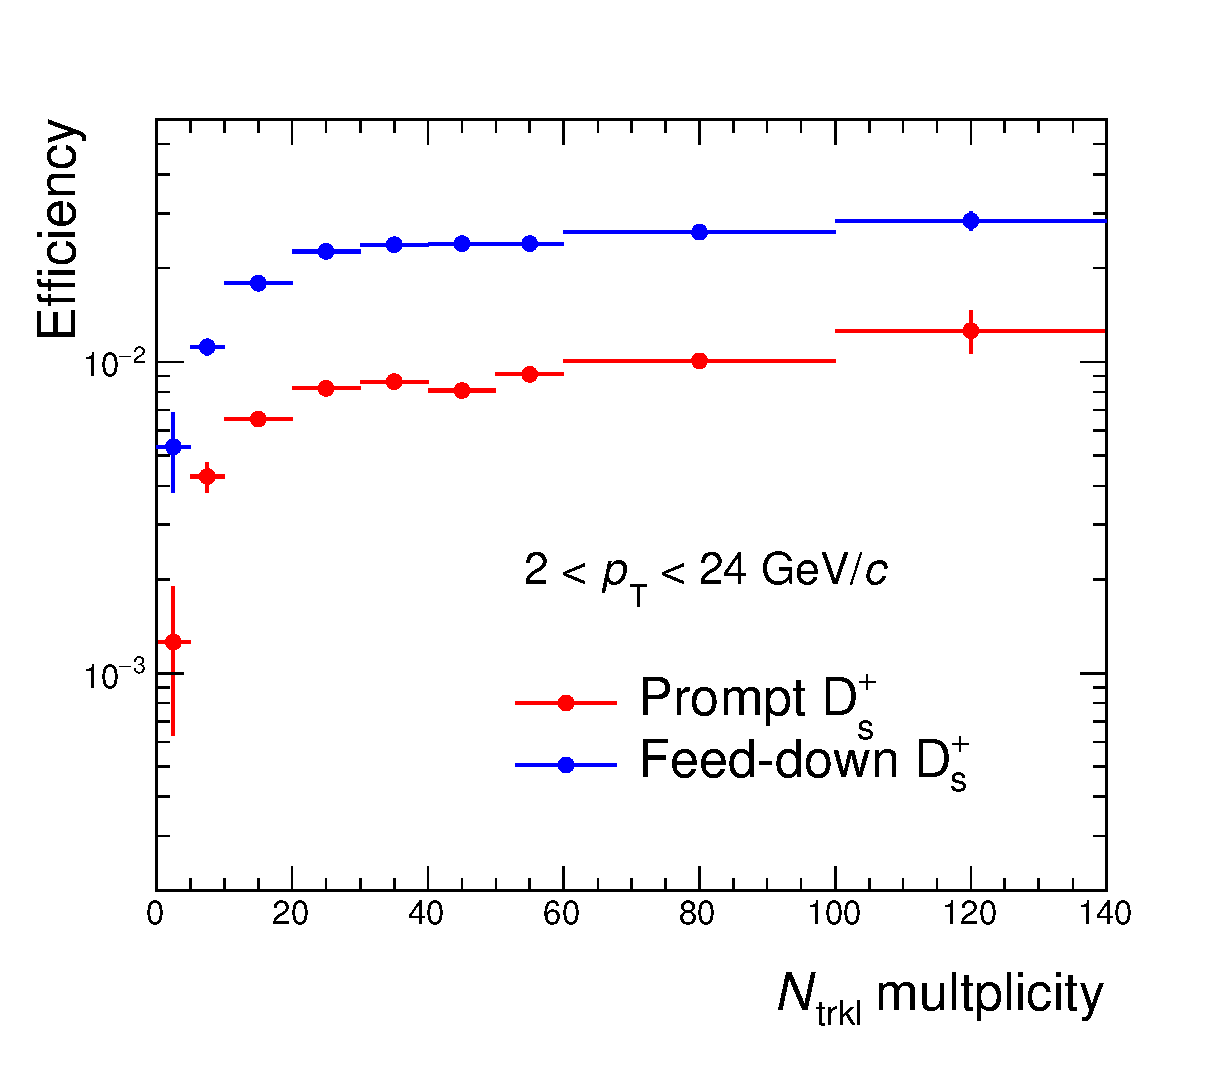
\includegraphics[width=.49\textwidth]{FigCap6/EffDsfineNtrklBins_Uncorr.eps}
 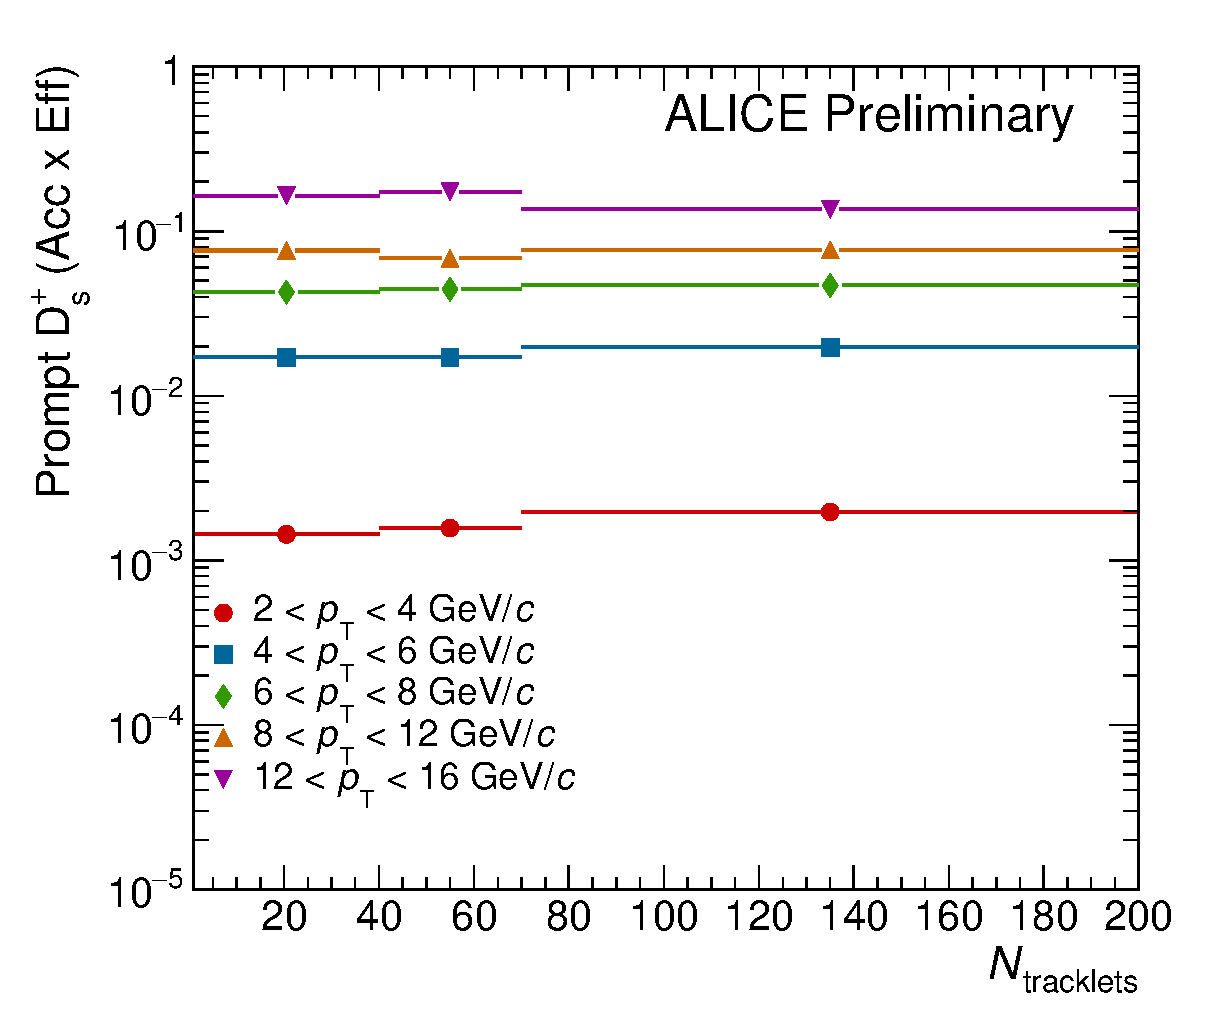
\includegraphics[width=.49\textwidth]{FigCap6/PromptDsEfficiency_times_Acceptance_VsNtrkl.eps}
 \caption{Left: $\Ds$ efficiency as a function of the tracklet multiplicity in fine intervals of $\Ntrkl$, for prompt (in red) and feed-down (in blue) $\Dsplus$. Right: $\Ds$ efficiency as a function of the tracklet multiplicity for the three $N_{\rm trkl}^{\rm corr}$ intervals used in the analysis, for the five $\pt$ intervals in different colours. The dashed lines represent the uncertainty band on $f_{\rm prompt}$.}
 \label{fig:DsEffVsMult}
\end{figure}



For the subtraction of the B feed-down contribution to the raw yields, the FONLL-based method 
described in Eq.~\ref{eq:fprAA} was used. It was 
assumed that the fractions of prompt $\Dsplus$ and $\Dplus$ do not depend on the 
multiplicity and therefore the prompt fractions computed in 
the multiplicity-integrated samples were used for all the $\Ntrkl$ classes. 
This hypothesis is supported by the results obtained for the D-meson nuclear modification factor 
analysis in different centrality classes~\cite{ALICEPAS2017008}, 
where the fractions of prompt D mesons in the 0-10\% and 60-100\%
centrality classes and in the minimum-bias sample were found to be compatible. 
In Eq.~\ref{eq:fprAA}, a hypothesis on $\RAA^{\rm feed-down}$
was applied to account for different modification of beauty and charm 
production in Pb-Pb collisions. In a similar way, for the calculation of $f_{\rm prompt}$ in 
the minimum-bias p-Pb sample, the assumption of $R_{\rm pPb}^{\rm feed-down} = R_{\rm pPb}^{\rm prompt}$ 
was done, for both $\Ds$ and $\Dplus$ mesons.
This hypothesis was varied between $0.9 <R_{\rm pPb}^{\rm feed-down}/R_{\rm pPb}^{\rm prompt} <1.3$ for the assignment of the systematic uncertainty. 
The resulting $f_{\rm prompt}$ for $\Dsplus$ mesons selected according to the criteria reported
in Tab.~\ref{tab:cutsDsVsNtrkl} is shown in Fig~\ref{fig:DsfPrompt} as a function of $\pt$.
%$0.9 < R_{\rm pPb}^{\rm feed-down} = R_{\rm pPb}^{\rm prompt} <1.3$ 
%to estimate the systematic uncertainty, as will be described in more details in the dedicated section. 

\begin{figure}[!h]
\centering
 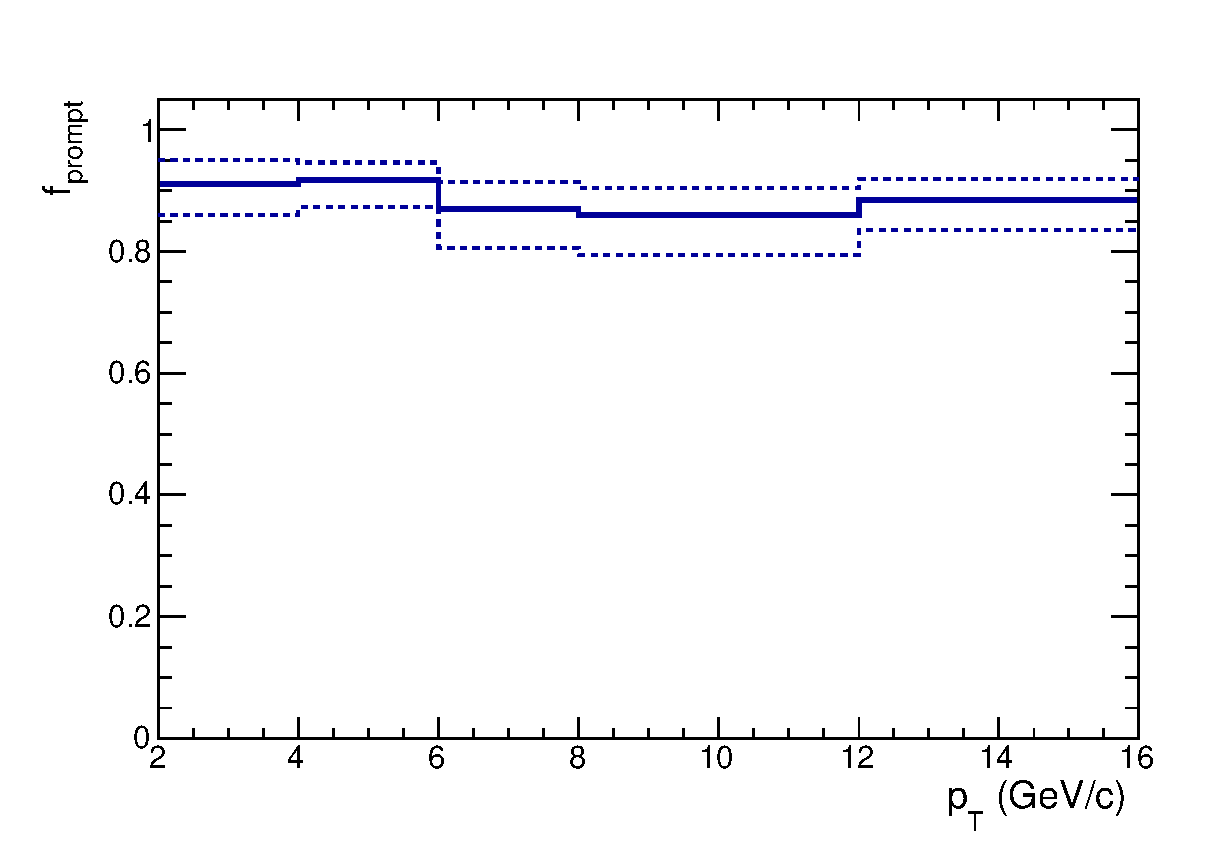
\includegraphics[width=.6\textwidth]{FigCap6/DsFprompt_1200Ntrkl.eps}
  \caption{Fraction of prompt $\Ds$ in the $\pt$ intervals considered for the analysis.}
 \label{fig:DsfPrompt}
\end{figure}

\section {Systematic uncertainties}
\label{sec:systpA}
Most of the sources of systematic uncertainty and the methodology for their evaluation are the same
that were discussed in Chapters~\ref{chap:pp} and~\ref{chap:PbPb} for
the pp and Pb-Pb analyses. They are the systematics on the yield extraction, 
the selection, on the efficiency (including $\Ds$ meson selection, track reconstruction and particle
identification) and on the generated D-meson $\pt$ shape.
The systematic uncertainty on the yield extraction was estimated via a multiple
trial approach by varying the configuration of the fit parameters and by comparing the
extracted yields with those using a bin counting method, as discussed in Sec.~\ref{sec:RawYieldSyst} and~\ref{sec:YieldExsystAA}. 
The systematic uncertainty on the selection efficiency was estimated by 
varying the topological selections applied on $\Ds$ candidates and testing the 
stability of the corrected yields in each $\pt$ interval (see Sec.~\ref{sec:CutVariation} and~\ref{sec:CutVarsystAA}). 
The systematic uncertainty on the particle
identification was assigned by comparing the corrected yields with the looser and tighter
PID selections introduced in Sec.~\ref{Sec:PID} and~\ref{sec:PIDsystPP}. 
The systematic uncertainty on the tracking efficiency was estimated by the comparison of the
efficiency in data and in simulation, after the data-driven re-weighting of the fraction of primary tracks in 
the simulation (see Sec.~\ref{sec:TrackEffSystPP}). 
The systematic uncertainty due to the generated $\Ds$-meson $\pt$ shape was estimated by considering different input
distributions (PYTHIA, FONLL) and was found to be negligible. As regards the systematic uncertainty on the calculation of the prompt 
fraction, the hypothesis on the $\RpPb$ of feed-down D mesons 
was varied in the range $0.9 <\RpPb^{\rm feed-down}/\RpPb^{\rm prompt} < 1.3$.
The error bars on $f_{\rm prompt}$ shown in Fig.~\ref{fig:DsfPrompt} include the
contribution of the variation of the hypothesis on $\RpPb^{\rm feed-down}$ 
as well as of the variation of factorisation and renormalisation scales and charm quark mass in FONLL. 
All the values of the assigned systematic uncertainties are reported
in Tab.~\ref{tab:DsVsMult_syst} as a function of $\pt$, for the 
three multiplicity classes. \\


An additional source of systematic uncertainty, which is specific of this analysis, is the one related to 
the re-weighting procedure of the efficiencies.  
Since the simulated $\Ntrkl$ distribution does not reproduce the distribution in data, 
a correction was introduced to re-weight the $\Ds$-meson efficiencies in each of the three $N_{\rm trkl}^{\rm corr}$ intervals, as described 
in Sec.~\ref{sec:Corrections}. 
The data-driven weights used for the central value of the efficiencies were obtained from
events that have at least a $\Dzero$-meson candidate
passing the selections, with invariant mass compatible within 3$\sigma$ to $\Dzero$ mass from PDG, as mentioned 
in Sec.~\ref{sec:Corrections}.
To estimate the systematic uncertainty on this procedure,
the efficiencies were corrected with weights from events that have at 
least a $\Dzero$-meson candidate, with no further request on its invariant mass. 
The two multiplicity dependent weights obtained in the two cases are shown in 
Fig.~\ref{fig:NtrklWeights_EvWithD_EvWithCand_Comparison} for the four groups of runs. 
Fig.~\ref{fig:DsDplusVsMult_SystEffWeights} shows the ratios of the efficiencies re-weighted 
with these two options for the multiplicity weights for the three intervals on $N_{\rm trkl}^{\rm corr}$ used
in the analysis. A 1\% systematic uncertainty was assigned based on the difference between 
the re-weighted efficiencies.\\

\begin{figure}[htpb]
\centering
 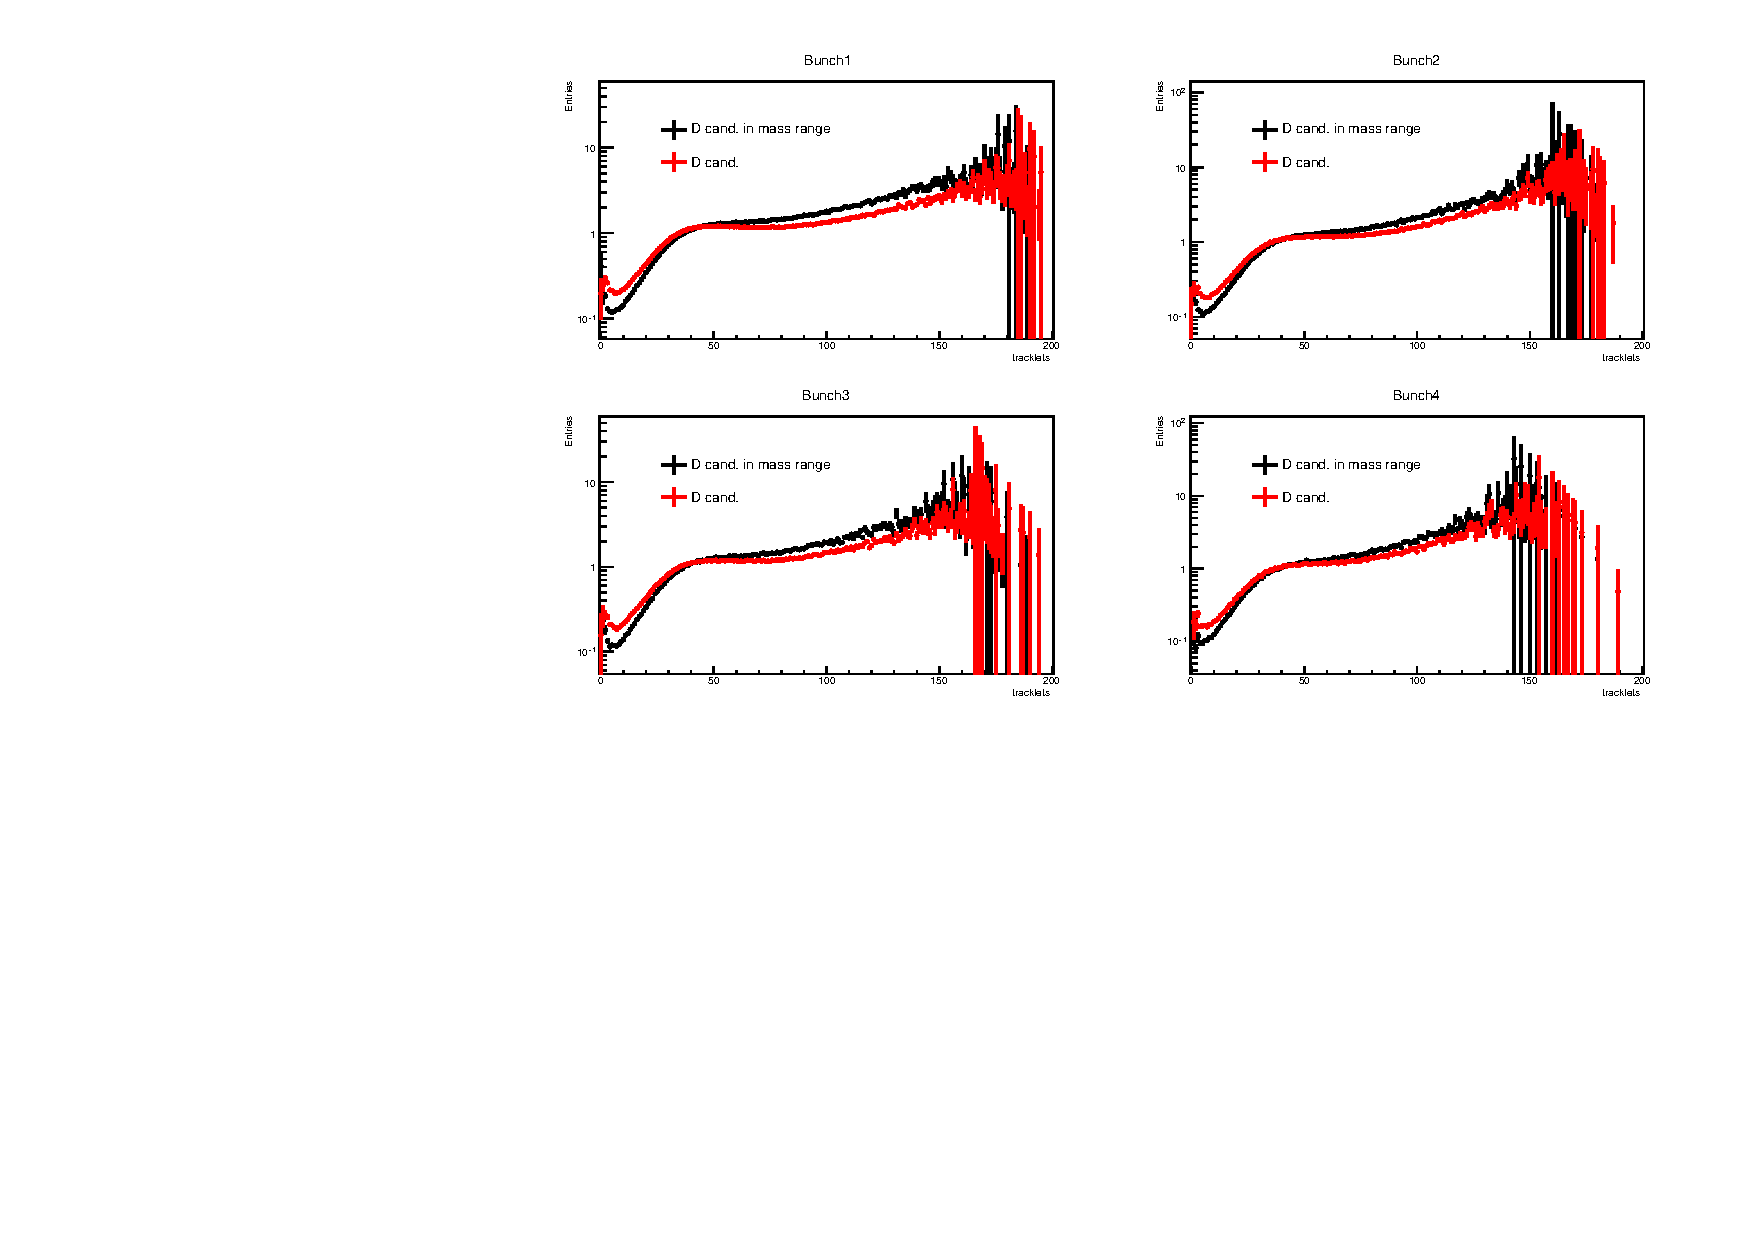
\includegraphics[width=.9\textwidth]{FigCap6/NtrkWeightsD-Cand_4Bunches_DsDplusVsmult.pdf}
 \caption{Comparison of the $\Ntrkl$ weights obtained from events with at least a $\Dzero$ candidate and from events with at least a $\Dzero$ candidate in the $\Dzero$ mass range (default).}
 \label{fig:NtrklWeights_EvWithD_EvWithCand_Comparison}
\end{figure}


\begin{figure}[htpb]
\centering
 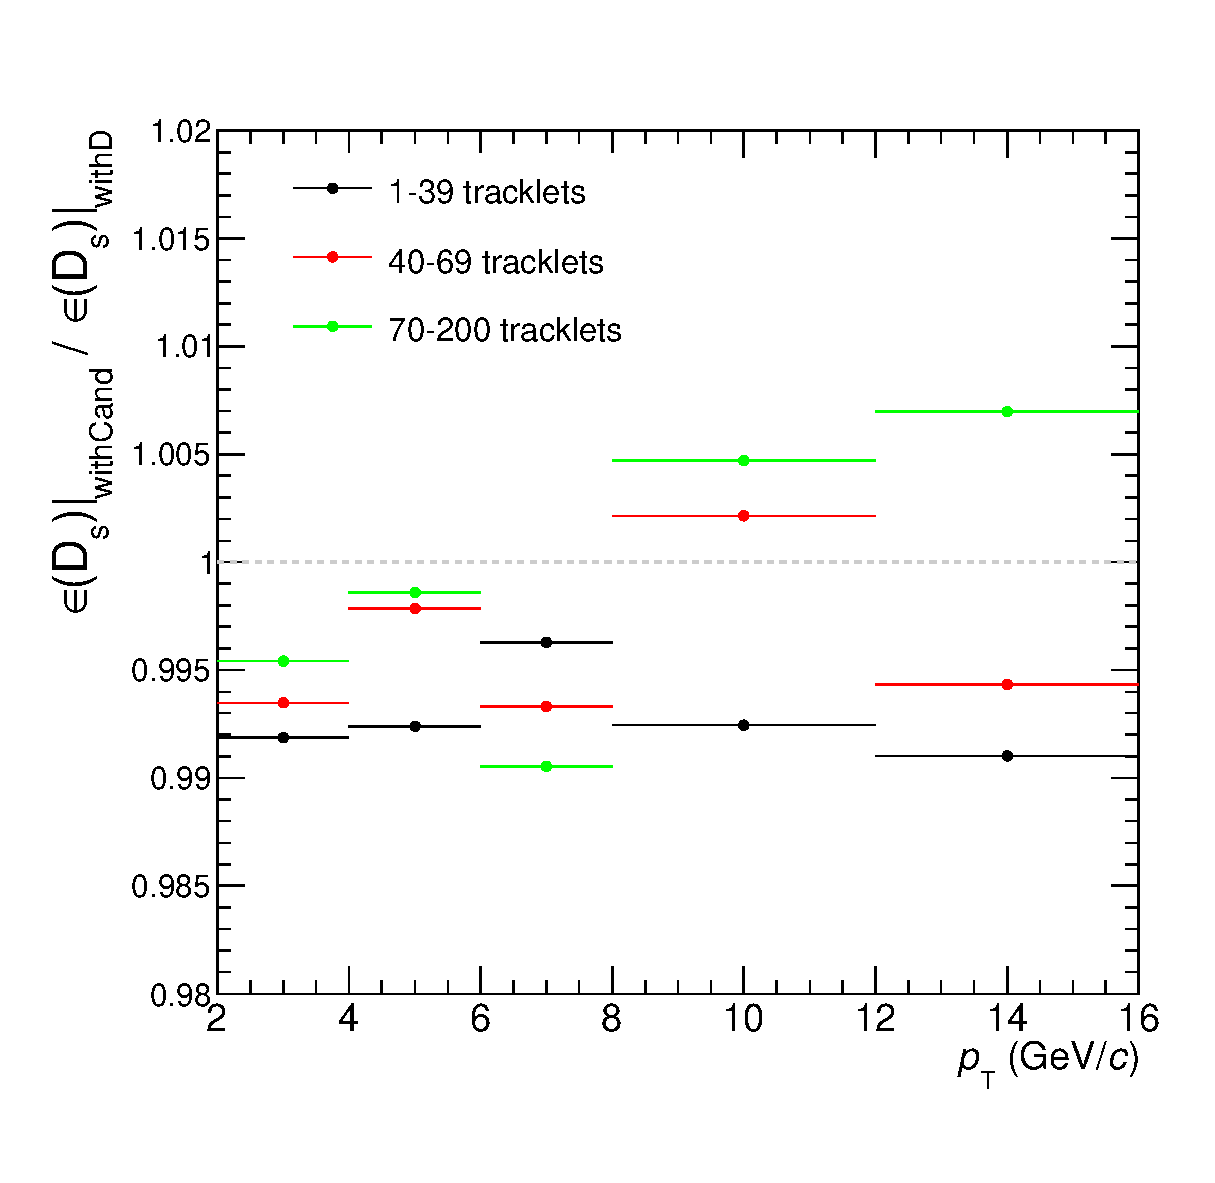
\includegraphics[width=.49\textwidth]{FigCap6/SystOnDWeightsWithCandVsWithD_Dsonly.eps}
 \caption{Ratio between the efficiency re-weighted with the two options considered for the $\Ntrkl$-dependent weights: events with 
 at least a $\Dzero$ candidate and events with at least a $\Dzero$ candidate in the $\Dzero$ mass range (default).}
 \label{fig:DsDplusVsMult_SystEffWeights}
\end{figure}



The same sources of systematic uncertainties were considered also for the $\Dplus$ meson.
In the calculation of the $\Ds/\Dplus$ yield ratios, the following sources of systematic 
uncertainties were considered as uncorrelated:
\begin{itemize}
\item raw-yield extraction;
\item selection efficiency;
\item PID selection efficiency;
\item hypothesis on $\RpPb^{feed-down}$ for the feed-down D meson subtraction;
\end{itemize}
while these other sources:
\begin{itemize}
\item efficiency correction with data-driven weights;
\item tracking efficiency;
\item variation of FONLL scales for the feed-down D meson subtraction;
\end{itemize} 
were considered as fully correlated between $\Dsplus$ and $\Dplus$ yields.


\begin{table}[h!]
\centering
\scalebox{0.9}{
\begin{tabular}{|l|c|c|c|c|c|}
\hline
 $\Ds$ syst. unc. (\%) & \multicolumn{5}{c|}{$\pt$ interval ($\GeV/c$)}\\
\hline
 $1 \leq \Ntrkl < 40$ & 2--4  & 4--6 & 6--8 & 8--12 & 12--16 \\
\hline
Yield extraction & 4 & 4 & 3 & 3 & 9\\
Selection efficiency  & 14   &   9   &     8	& 8	&7\\
PID efficiency &  2 & 2 & 2 & 2 & 2 \\
Tracking efficiency & 4 & 4 & 4 & 4 & 4 \\
MC $\pt$-shape & negl & negl & negl & negl & negl \\
Feed-down  &	$^{+3}_{-4}$	& $^{+3}_{-4}$ & $^{+3}_{-4}$ & $^{+3}_{-4}$	&$^{+5}_{-5}$\\
Multiplicity weights & 1 &  1 &  1 &  1 &  1 \\
\hline
 $40 \leq \Ntrkl < 70$ & 2--4  & 4--6 & 6--8 & 8--12 & 12--16 \\
\hline
Yield extraction & 3 & 3 & 4 & 5 & 12\\
Selection efficiency & 14 & 9 & 8	& 8	&7\\
PID efficiency&  2 & 2 & 2 & 2 & 2 \\
Tracking efficiency& 4 & 4 & 4 & 4 & 4 \\
MC $\pt$-shape & negl & negl & negl & negl & negl \\
Feed-down  &	$^{+3}_{-4}$	& $^{+3}_{-4}$ & $^{+3}_{-4}$ & $^{+3}_{-4}$	&$^{+5}_{-5}$\\
Multiplicity weights & 1 &  1 &  1 &  1 &  1 \\
\hline
 $70 \leq \Ntrkl < 200$ & 2--3  & 4--6 & 6--8 & 8--12 & 12--16 \\
\hline
Yield extraction   & 4 & 4 & 4 & 4 & 10\\
Selection efficiency & 14 & 9 & 8	& 8	&7\\
PID efficiency&  2 & 2 & 2 & 2 & 2 \\
Tracking efficiency& 4 & 4 & 4 & 4 & 4 \\
MC $\pt$-shape & negl & negl & negl & negl & negl \\
Feed-down  &	$^{+3}_{-4}$	& $^{+3}_{-4}$ & $^{+3}_{-4}$ & $^{+3}_{-4}$	&$^{+5}_{-5}$\\
Multiplicity weights & 1 &  1 &  1 &  1 &  1 \\
\hline
\end{tabular}}
\caption{Systematic uncertainties on $\Ds$ yield used in the $\Ds/\Dplus$ versus multiplicity measurement.}
\label{tab:DsVsMult_syst}
\end{table}

\section {Conversion of $\Ntrkl$ to primary charged particles}
\label{sec:NtrklToNch}
The conversion of the number of tracklets in $|\eta|<1$ to the average multiplicity of primary charged particles ($\Nch$) 
in the same $\eta$ range was performed using a Monte Carlo production with the EPOS-LHC generator~\cite{Drescher:2000ha}. 
The distribution of the reconstructed $\Ntrkl$ as a function of the number of
$\Nch$ in the simulation, which is shown in Fig.~\ref{fig:NtrklVsNch} (left), was considered to this purpose.
The 2D correlation was re-weighted with the $\Ntrkl$ weights obtained
as the ratio of the $\Ntrkl$ distributions in data and in simulation as described in 
Sec.~\ref{sec:Corrections}, to adapt the tracklet distribution from the simulation to that of the data.
The $\Ntrkl$ distributions were obtained with the request of at least a $\Dzero$ candidate
in the $\Dzero$ mass range. 
The profile of the correlation was fitted with a linear function with two parameters $\Ntrkl={\rm a}+{\rm b} \Nch$.
The parameters were found to be: a $=(-0.3 \pm 0.1)$ and b $=(0.900\pm 0.002)$. The profile-to-fit ratio
is presented in Fig.~\ref{fig:NtrklVsNch} (right panel). The fitted function was used 
to extract the central value of $\averNch$ from the average $\averNtrkl$ value in each class. \\



To estimate the systematic uncertainties on the evaluation of the average 
$\Nch$ values in the considered $\Ntrkl$ intervals, three different checks have been performed.
\begin{enumerate}
\item To test the dependence of the correction factor on the event generator, the correlation between
$\Ntrkl$ to $\Nch$ with a different event generator (DPMJET~\cite{Ranft:1994fd}) was considered. The correlation
between $\Ntrkl$ to $\Nch$ can in fact be sensitive to the relative abundance of different particle species
produced by the event generator. The comparison of the average $\Nch$ in the three $\Ntrkl$ intervals
used in the analysis from the EPOS and DPMJET generators
is presented in Fig.~\ref{fig:NchVsMCgenerator}. The difference, which is 2\% in all $\Ntrkl$ intervals,
was assigned as systematic uncertainty.
\item To test deviations from the linear correlation which were observed in particular at low and high multiplicity (right panel of Fig.~\ref{fig:NtrklVsNch}), a different method to compute $\averNch$ was considered.  
The average $\Nch$ was extracted by considering the $\Nch$ intervals used in the analysis as shown in Fig.Fig.~\ref{fig:NtrklProj}.
In Fig.~\ref{fig:NchVsCorrHypo} (left) the comparison of the $\averNch$ values
obtained with this methods are compared to the ones computed with the linear fit. The difference
is $<3\%$ in all $\Ntrkl$ intervals and is assigned as systematic uncertainty.
\item To estimate the dependence on the shape of the multiplicity distribution,
the conversion factor from $\Ntrkl$ to $\Nch$ was recalculated: (i) without the data-driven 
$\Ntrkl$ weights and (ii) applying the $\Ntrkl$ weights obtained considering all 
the events that pass the physics selection, without requirements on the 
$\Dzero$ candidate. The comparison of $\averNch$ values from these tests to the default one, 
obtained with the weights extracted from events with $\Dzero$ candidates in the $\Dzero$ mass range, 
is shown in Fig.~\ref{fig:NchVsCorrHypo} (right). The assigned systematics are $5\%, 0\%, 3\%$ in the 
$[1,40), [40,70), [70,200]$ $\Ntrkl$ intervals respectively.
\end{enumerate}
The three sources of uncertainties were considered as 
uncorrelated and their contributions were summed in quadrature. The final values of $\averNch$ in $|\eta|<1$ 
and the associated systematic uncertainties are shown in 
Fig.~\ref{fig:Nch}. These values were then divided by the 
width of the considered $\eta$ range, $\Delta \eta =$ 2, 
to obtain $\langle {\rm d} \Nch/{\rm d}  \eta \rangle |_{|\eta|<0.5}$.\\


\begin{figure}[h]
\centering
 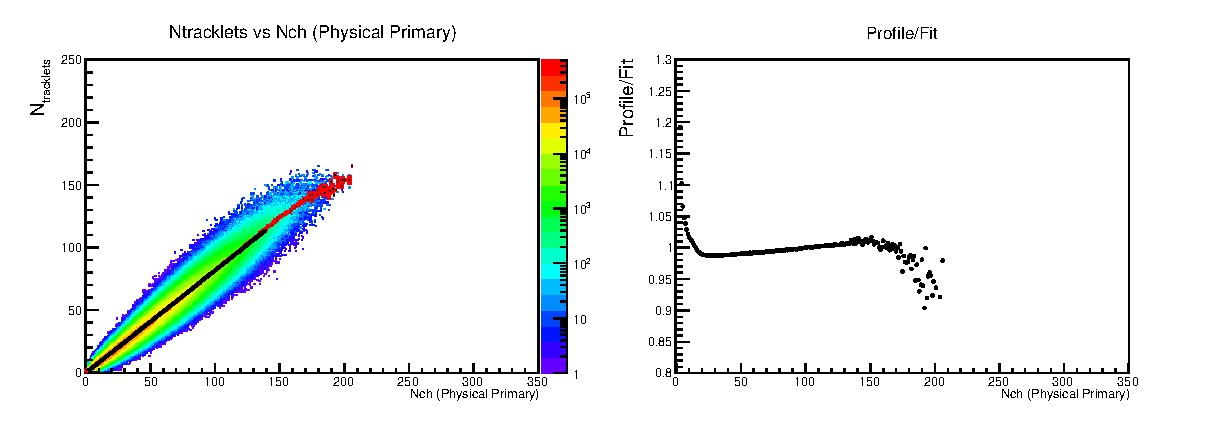
\includegraphics[width=1.\textwidth]{FigCap6/NtrklVsNchPhysPrimWithNtrklsReweight17f2a.eps}
 \caption{Left: distribution of number of SPD tracklets $\Ntrkl$ versus number of generated charged particles $\Nch$ obtained from simulations with the EPOS-LHC generator. The profile of the correlation (red markers) is fit with a linear function (black line). Right: ratio of the profile of $\Ntrkl$ versus $\Nch$ distribution to the fit result.}
 \label{fig:NtrklVsNch}
\end{figure}

\begin{figure}[!h]
\centering
 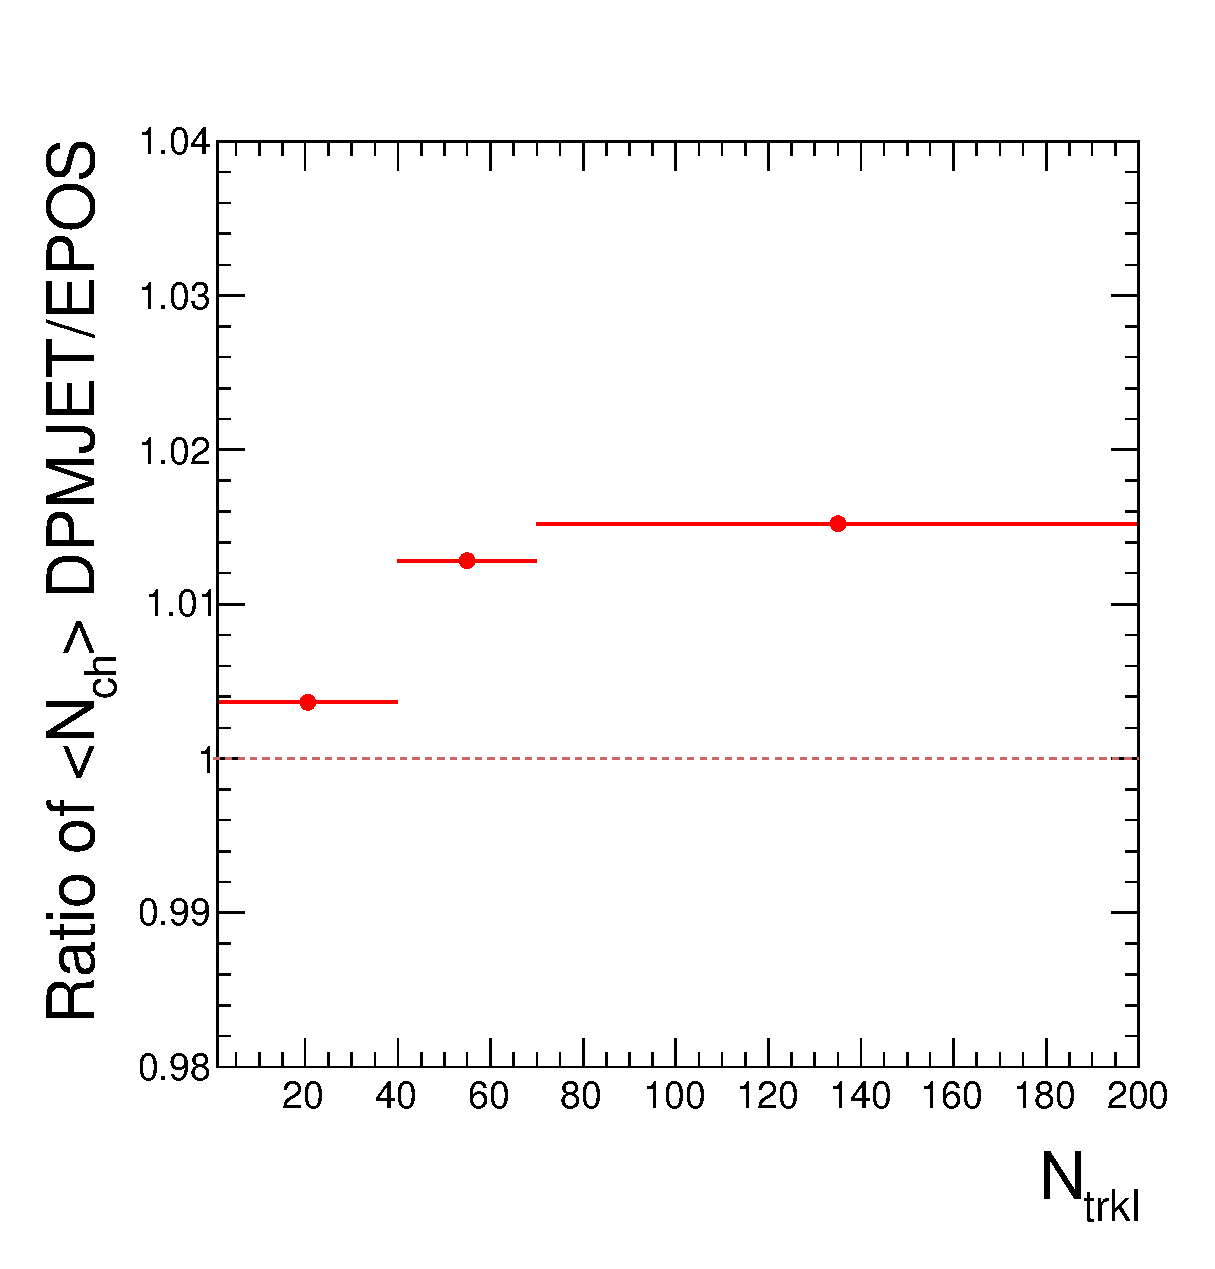
\includegraphics[width=.49\textwidth]{FigCap6/comparisonNtrkl_17f2b_17d2a_17f2a_onlySyst.eps}
 \caption{Ratio of $\averNch$ values in the considered multiplicity classes obtained with EPOS-LHC and DPMJET generators.}
 \label{fig:NchVsMCgenerator}
 \end{figure}

\begin{figure}[!h]
\centering
 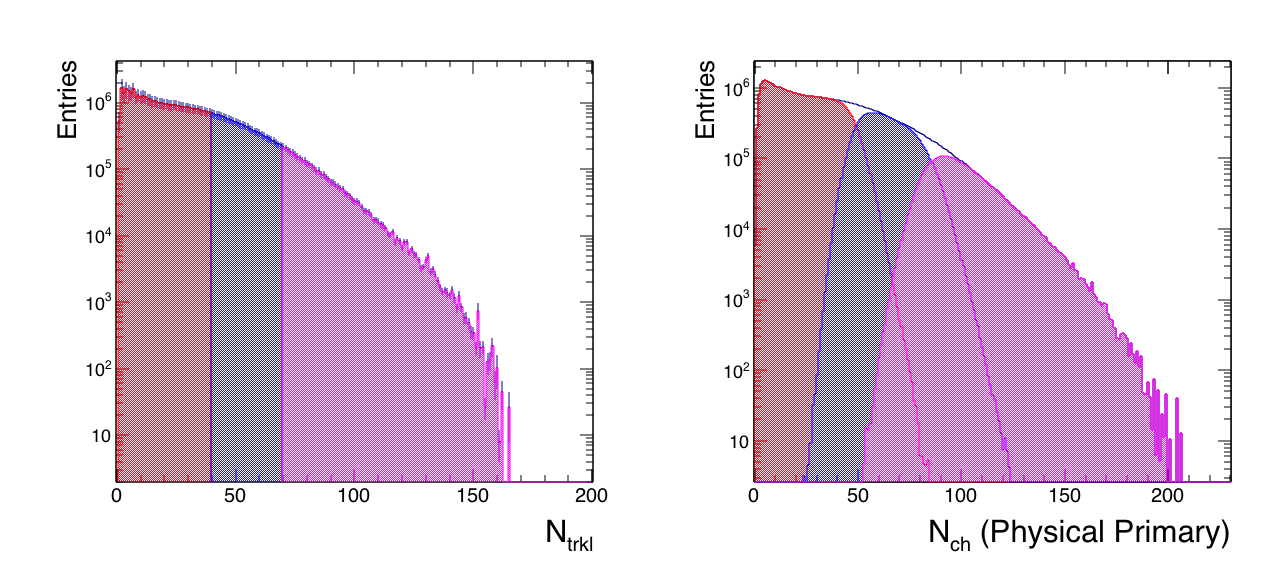
\includegraphics[width=1.\textwidth]{FigCap6/NtrklNchDistrWithNtrklsReweight_17f2a.png}
 \caption{Left: $N_{\rm trkl}^{\rm corr}$ distributions for the three multiplicity classes from simulations with EPOS-LHC. Right: $\Nch$ distributions 
 in the three multiplicity classes.}
 \label{fig:NtrklProj}
\end{figure}

\begin{figure}[!h]
\centering
 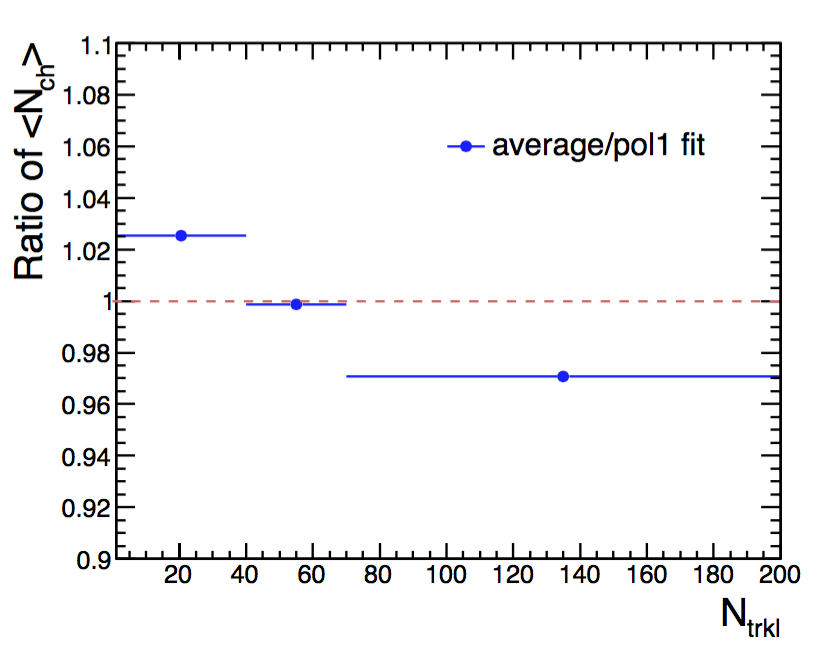
\includegraphics[width=.49\textwidth]{FigCap6/NchSystematics_linFit_WithNtrklsReweight_17f2a.png}
 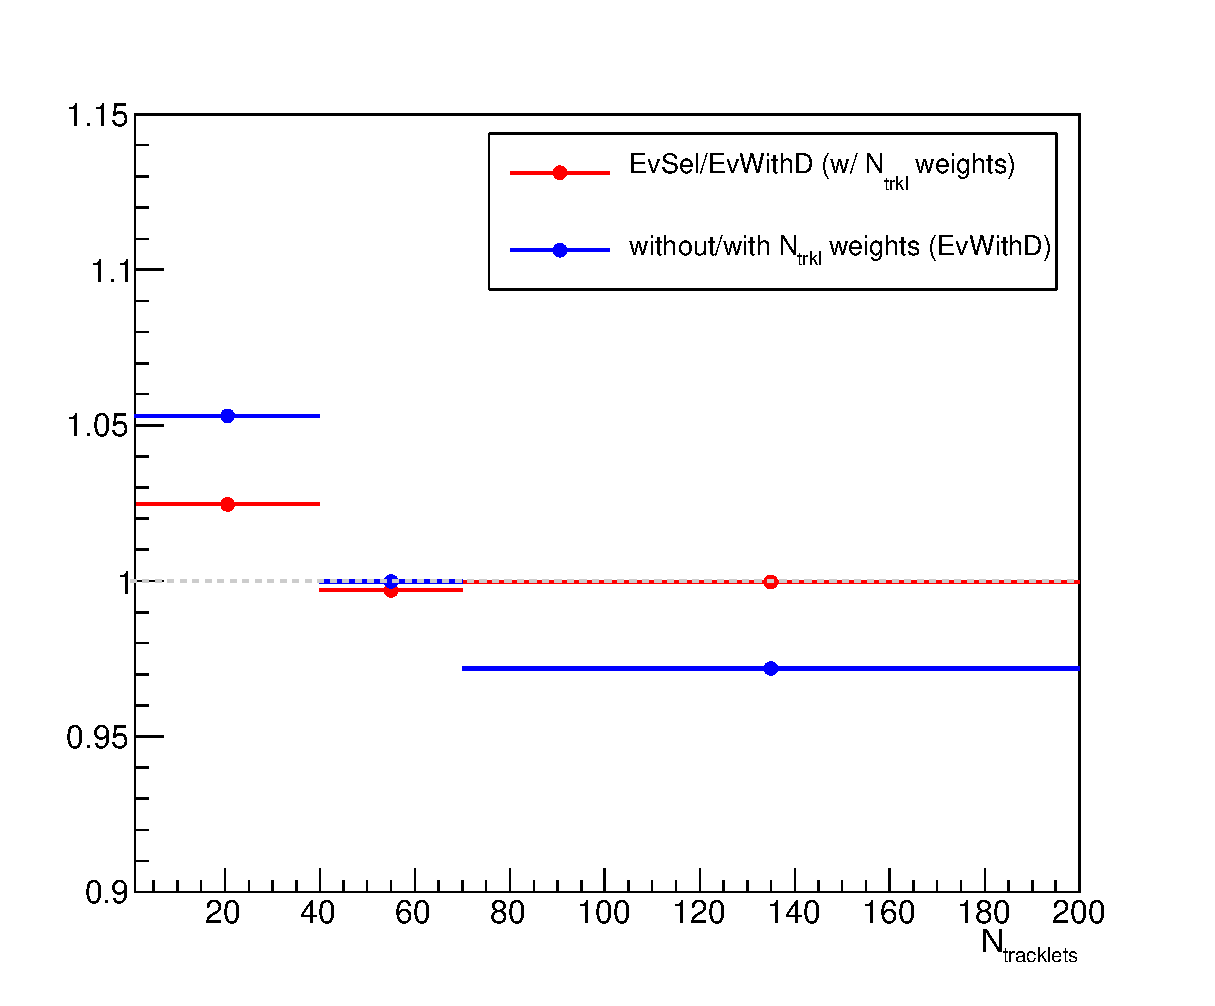
\includegraphics[width=.49\textwidth]{FigCap6/NchSystematics_NtrklWeights_17f2a.eps}
 \caption{Left: ratio of $\averNch$ values obtained as average of the $\Nch$ distributions in the $\Ntrkl$ intervals to those obtained from the linear fit to the $\Ntrkl$-$\Nch$ correlation. Right: ratios of $\averNch$ values obtained with different data-driven weights.}
 \label{fig:NchVsCorrHypo}
 \end{figure}

\begin{table}[h!]
\centering
\scalebox{0.9}{
\begin{tabular}{c|c|c|c}
\hline
\hline
$\averNch$ & $\Ntrkl$ weights (\%)   & Lin. corr. $\Ntrkl$-$\Nch$  (\%)& Ev. generator  (\%)\\ 
\hline
21.6     &   6.9  &  2.6 &  0.4 \\
63.1     &   0.7  &  0.1 &  1.3 \\
102.7   &   2.5  &  2.9 &  1.5 \\
\hline
\end{tabular}}
\caption{Systematic uncertainties on $\averNch$ values in each of the three $\Ntrkl$ multiplicity intervals.}
\label{tab:DsVsMult_syst}
\end{table}

\begin{figure}[h]
\centering
 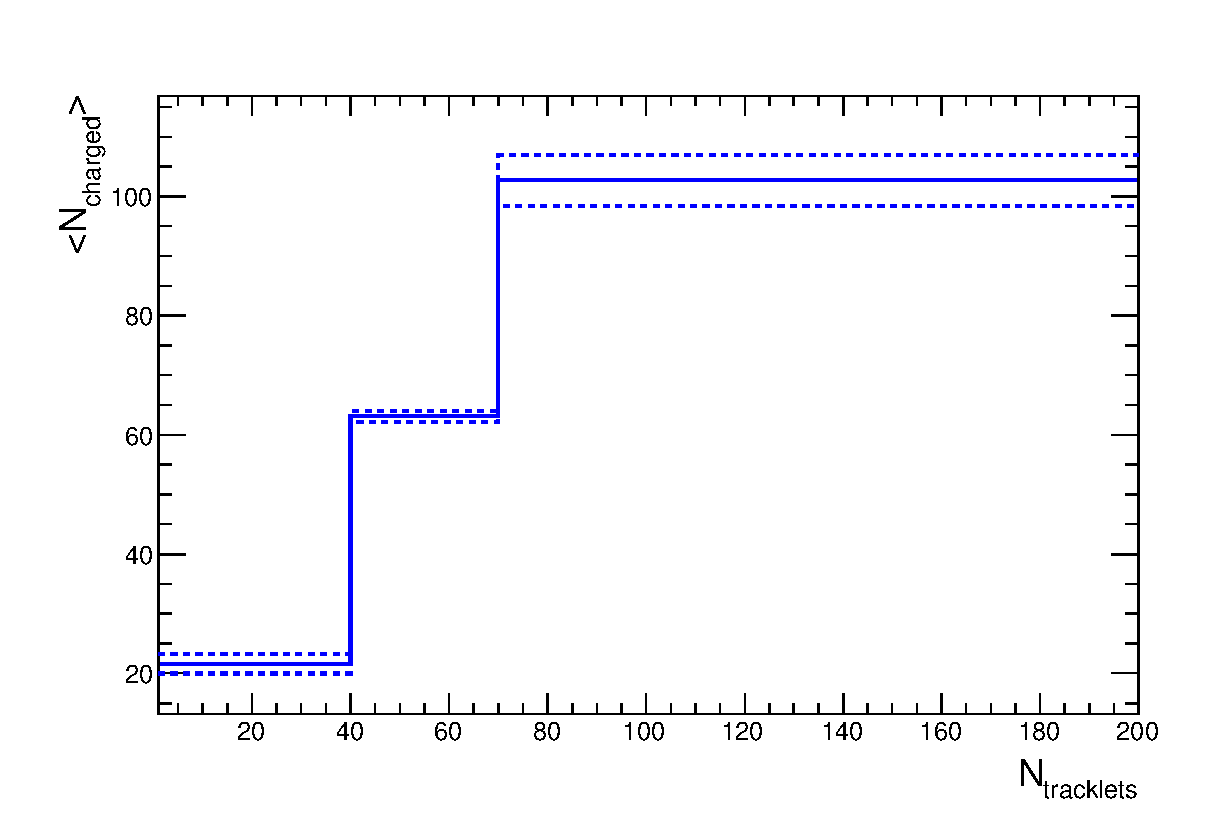
\includegraphics[width=.55\textwidth]{FigCap6/AverNchAndTotalSystUnc.eps}
 \caption{Average $\Nch$ values in $|\eta|<1$ for the considered multiplicity classes. The lower and higher dashed lines represent the systematic uncertainties.}
 \label{fig:Nch}
\end{figure}

\section{Results}
\label{sec:results}
The ratios of $\Ds/\Dplus$-meson yields are shown in Fig.~\ref{fig:DsDplusRatios} as a function of
the average number of primary charged particles per unity of pseudo-rapidity, 
in five $\pt$ intervals from 2 to 16 $\Gevc$.
The ratios measured in pp collisions at $\sqrt{s}=$7 TeV~\cite{Acharya:2017jgo} and 
in Pb-Pb collisions at $\sqrt{s_{\rm NN}}=$ 5.02 TeV~\cite{ALICE-PUBLIC-2017-003}
(for the 0-10\%, 30-50\% and 60-100\% centrality classes), which were presented in Chap.~\ref{chap:pp} and~\ref{chap:PbPb} 
are also reported in the figure.
A hint for an enhanced $\Ds/\Dplus$ ratio in Pb-Pb collisions was discussed in Chap.~\ref{chap:PbPb} and could result
from a significant contribution of recombination mechanism in charm-quark hadronisation in the QGP.
The data point in Fig.~\ref{fig:DsDplusRatios} could provide further insight on the multiplicity 
dependence of this possible enhancement also in the smaller systems, such as those produced
in p-Pb collisions. The measured $\Ds/\Dplus$ ratios in p-Pb collisions in the different 
multiplicity and $\pt$ intervals are found to be compatible within uncertainties. 
To test for possible presence of non-flat trends as a function of multiplicity, the measured points were 
fitted with a linear function to quantify their slope. The results of the fit are shown in Fig.~\ref{fig:FitRatios}
and were obtained considering only the statistical uncertainties. The reason for this choice is that, without including the
systematic uncertainties, the slopes from the linear fit on the pp, 
p-Pb and Pb-Pb points were found to be different from zero already no more than 
1$\sigma$ of the slope parameter error between 2 and 8 $\Gevc$. 
If the fit is performed on pp and p-Pb measurements only (blue lines in Fig.~\ref{fig:FitRatios}), 
the slopes differ from zero within 1$\sigma$ 
in the $\pt$ intervals between $4<\pt<6 \, \Gevc$ and $6<\pt<8 \,\Gevc$. 
 
\begin{figure}[h!]
    \begin{center}
          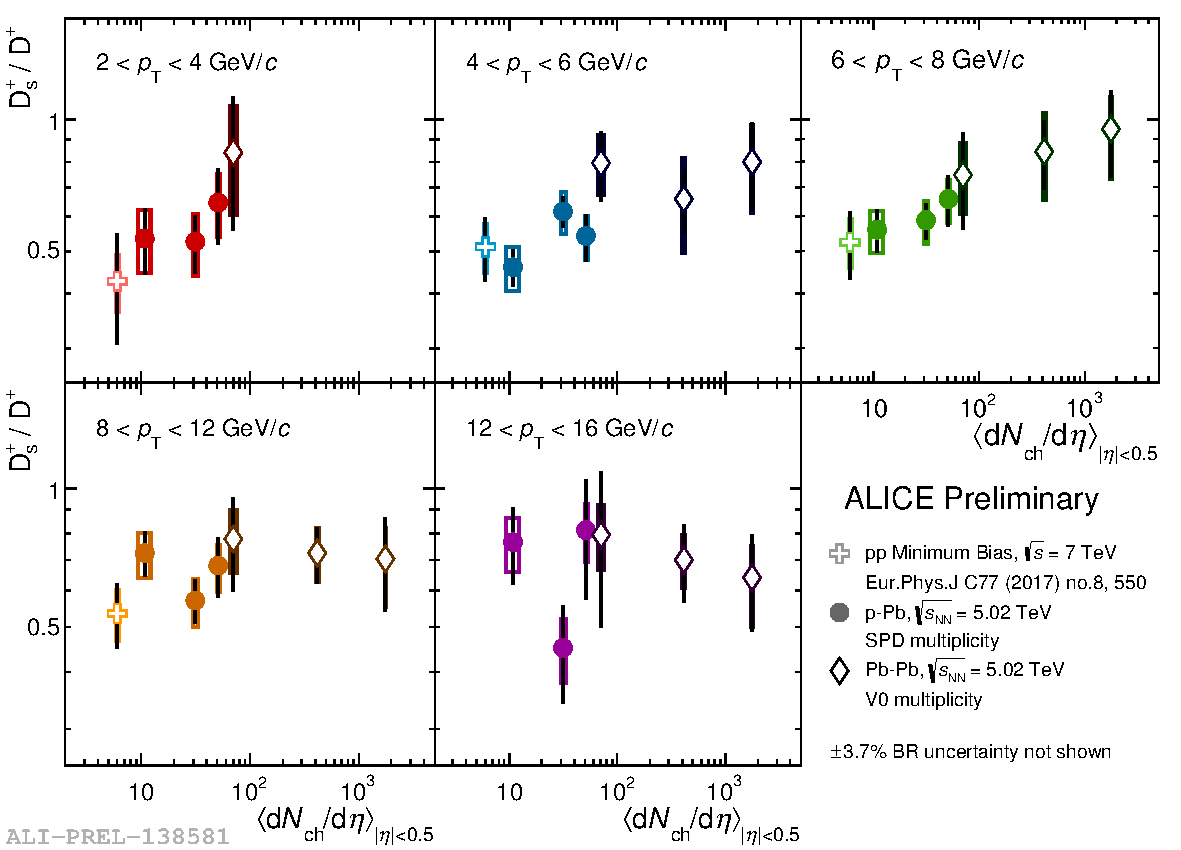
\includegraphics[width=1\textwidth]{./FigCap6/DsOverDplusVsMult_pp_pPb_PbPb.pdf}
    \end{center}
    \caption{ $\Ds/\Dplus$-meson yield ratios as a function of the multiplicity of primary charged particles in $|\eta|<0.5$, in the five $\pt$ intervals from 2 to 16 $\Gevc$.}
    \label{fig:DsDplusRatios}
\end{figure}

\begin{figure}[h!]
    \begin{center}
          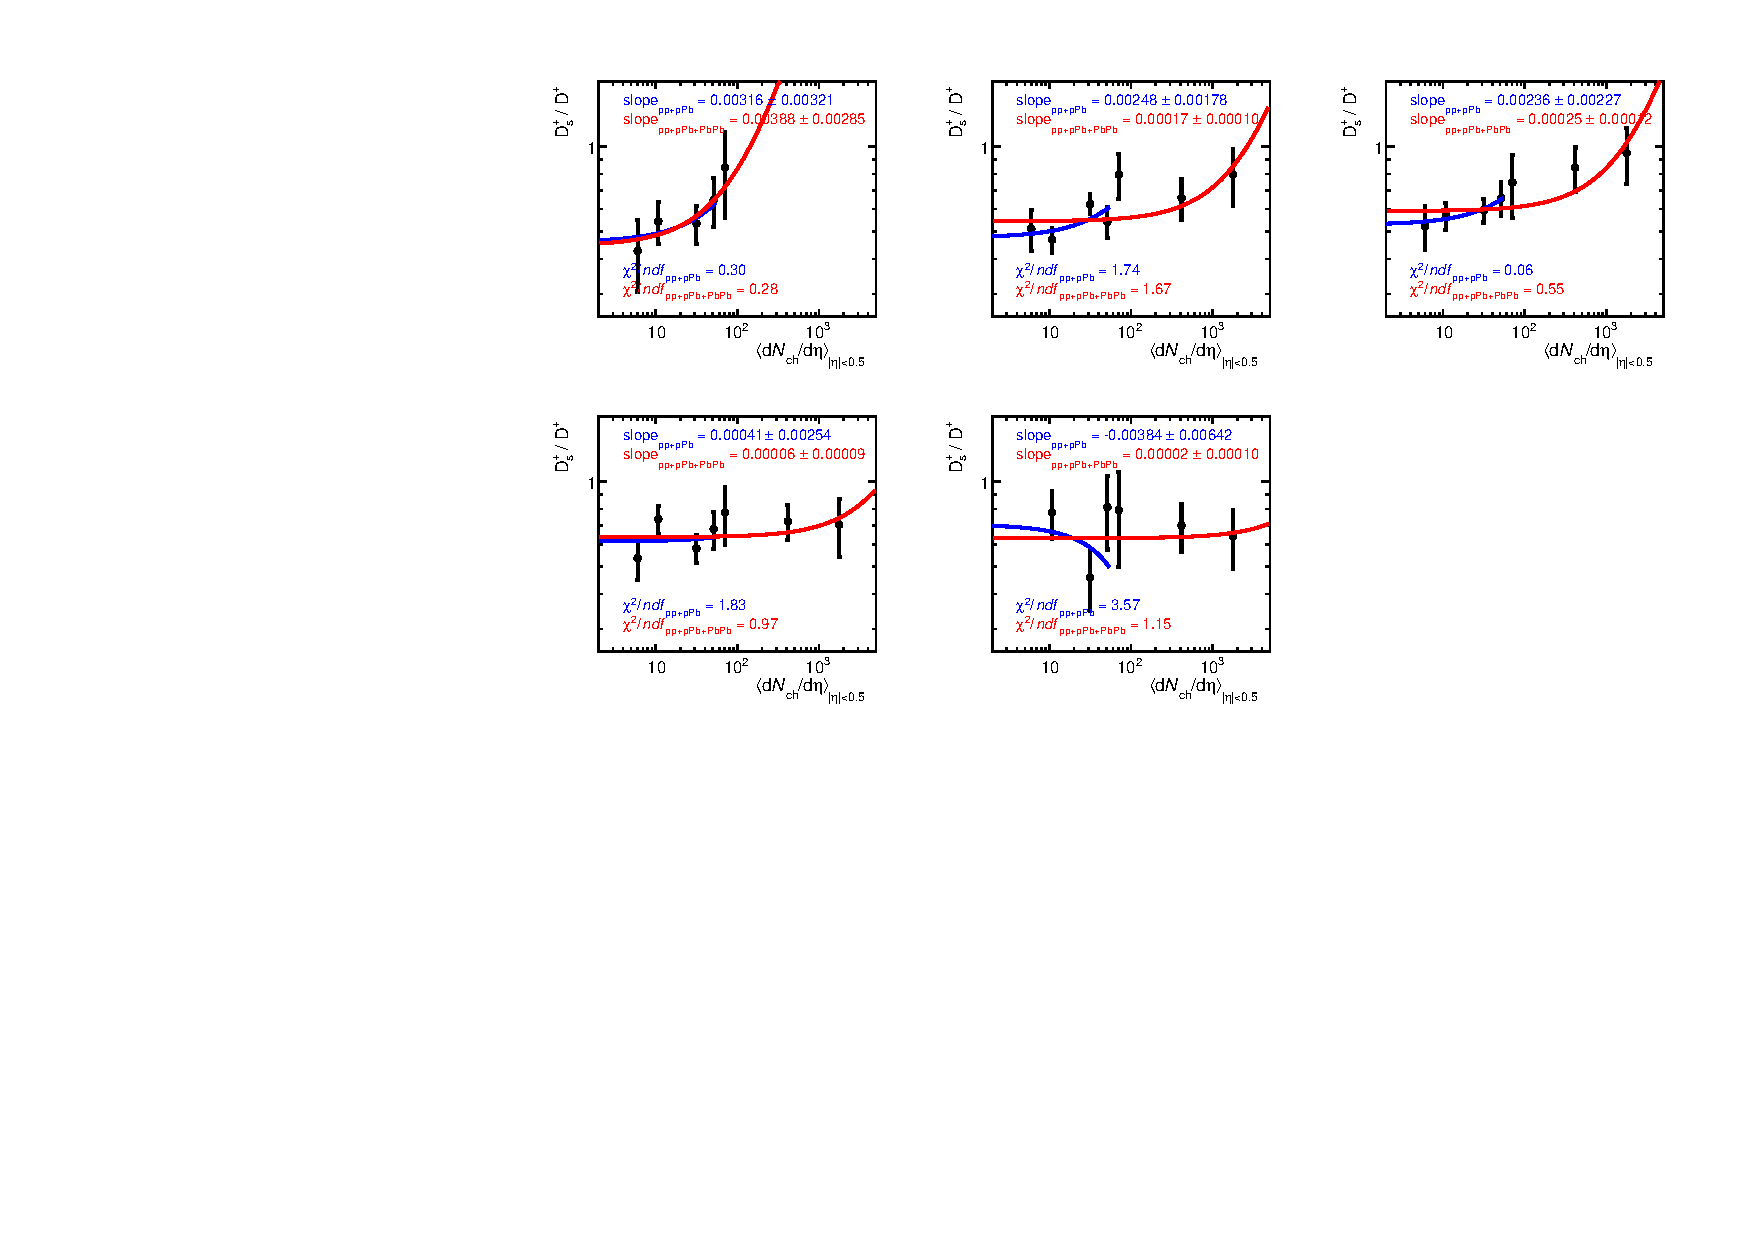
\includegraphics[width=1.1\textwidth]{./FigCap6/Fit_DsOverDplusVsMult_pp7TeV_pPb5TeV_PbPb5TeV.pdf}
    \end{center}
    \caption{Linear fit to $\Ds/\Dplus$ ratios as a function of the multiplicity of primary charged particles, in the different $\pt$ intervals from 2 to 16 $\Gevc$. The slope parameter of the linear function is reported in each pad, for the fits made only on the pp and p-Pb points (blue lines) or on
    all the pp, p-Pb and Pb-Pb points (red lines). Only statistical uncertainties are considered in the fit.}
    \label{fig:FitRatios}
\end{figure}


\section{Discussion and perspectives}
\label{sec:discussionpPb}
The measured hint of $\Dsplus/\Dzero$ and $\Dsplus/\Dplus$ in Pb-Pb collisions at $\sNN=5.02$ TeV
that was discussed in Chap.~\ref{chap:PbPb} is expected in case of charm-quark hadronisation
via recombination in the QGP. Experimental observations in high-multiplicity pp collisions and in p-Pb collisions that resemble
effects observed in Pb-Pb collisions (long-range rapidity correlations, measurements of azimuthal anisotropies $v_n$ ...) (see Chap.~\ref{Chapter1}) 
were found.
It is not clear yet which is the physics behind these observations, for which 
explanations based on collectivity effects and also on the formation of droplets of QGP in small systems were proposed.
The measurement of $\Dsplus/\Dplus$ yield ratios is a test for the possible presence of charm-quark recombination
also in small systems (high multiplicity pp and p-Pb collisions). Although intriguing, 
the current measurement of $\Dsplus/\Dplus$ as a function of the multiplicity in p-Pb collisions does
not allow to draw firm conclusions due to the large statistical and systematic uncertainties.\\




The precision of this measurement will be improved using the 
larger data samples of p-Pb collisions that will be collected during the LHC Run 3.
Fig.~\ref{fig:DsEstimatespPb} shows the estimate for the relative systematic uncertainty of 
$\Ds$ yield in minimum-bias p-Pb collisions at $\sNN=$ 5.5 TeV estimated for Run 3, and compared to Run 2 preliminary results~\cite{ALICE-PUBLIC-2017-008}. 
During LHC Run 3, a sample of $\sim 150$ times the current one could be recorded. 
The estimates in Fig.~\ref{fig:DsEstimatespPb} were obtained by rescaling the statistical 
uncertainty on the production yield from the current sample to the statistics expected for Run 3 for $\pt>2\,\Gevc$ (full red markers). 
The statistical uncertainties are expected to be 1\% or less for $\pt>2\,\Gevc$.
For the low-$\pt$ region, the estimates were obtained from an analysis of $\Dsplus$ production without secondary vertex
reconstruction (open red symbols). Since the $\Ds$-meson decay topology cannot be efficiently resolved at low $\pt$ due to the 
insufficient resolution of the track impact parameter and the small Lorentz boost, all the selections
based on the secondary-vertex topology were not applied.
Since it is impossible to have a measurement of the $\Dspm$ signal from the data of p-Pb in Run 2 
due to the large amount of background at $\pt<2\,\Gevc$, the signal was obtained as:
\begin{equation}
\begin{split}
\label{eq:sigStime}\
S_{{\rm D}_{s}^+}\big|_{\rm p-Pb, 5 TeV} = \, \langle {\rm T}_{\rm pA}^{\rm \,0-100\%}\rangle\,\sigma_{\rm FONLL}^{\rm{ D}^{\rm 0},pp, 5 TeV} \,\frac{{\rm d}N^{\rm{ D}{\rm s}^+,pp 7 TeV}/{\rm d}\pt}{{\rm d}N^{\rm{ D}^{\rm 0}, pp 7 TeV}/{\rm d}\pt}\, \times ({\rm Acc\times \epsilon})_{{\rm D_s}^+}^{\rm p-Pb, 5 TeV}\\
\times \,2\,{\rm BR(\DstoKKpi)}\, ,
\end{split}
\end{equation}
where $\sigma_{\rm FONLL}^{{\rm D}^{\rm 0,pp, 5 TeV}}$ is the FONLL cross-section at $\sNN=5$ TeV for $\Dzero$ meson
production, which was rescaled to $\Dsplus$ cross section with the ratio of the $\Dsplus/\Dzero$ yields measured 
in pp collisions at $\s=7$ TeV (see Chap.~\ref{chap:pp}). This ratio was found to be $\sim 0.2$ between $2 <\pt <12 \, \Gevc$
and assumed to be constant at $\pt<2\,\Gevc$. Results of $\Dsplus/\Dzero$ yields in p-Pb collisions at $\sNN=5.02$ TeV~\cite{ALICE-PUBLIC-2017-008}
are compatible with those in pp collisions used here.
The cross-section was then rescaled by the average nuclear overlap function 
$\langle {\rm T}_{\rm pA}^{\rm \,0-100\%}\rangle$ in p-Pb collisions at  $\sNN=5$ TeV and by the $({\rm Acc\times \epsilon})_{{\rm D_s}^+}^{\rm p-Pb, 5 TeV}$ term calculated from the simulations to converted the cross section into a yield. To calculate the $({\rm Acc\times \epsilon})$, only 
the selections on $\cos \theta^*(\pi)$, $|\cos^3 \theta^\prime({\rm K})|$ and on the
invariant mass of the reconstructed K$^+$K$^-$ pair were used. Finally, the yield was rescaled for the 
branching ratio of $\DstoKKpi$. The factor 2 accounts for particle and charge conjugate production.
The background contribution was obtained from data by integrating the amount of candidates 
obtained with the same selections used for the efficiencies within 3$\sigma$ of the simulated 
peak width from the $\Ds$ invariant mass value. The estimates for the signal and the background
were combined into a statistical significance. The relative uncertainty on the signal can be obtained 
from the significance value: $\delta S/S \sim 1/{\rm significance}$. The statistical uncertainty was finally scaled
by the number of events that could be recorded in Run 3.\\



The upgrade ITS that will be installed after Run 2 will allow to further improve the statistical uncertainty from 
the estimates discussed above, thanks to its improved resolution on primary and secondary vertex reconstruction.
This will paves the way to measure with sufficient precision the $\Dsplus$ production as a function of the multiplicity
in small systems and to assess about how the charm hadronisation evolves from pp to Pb-Pb collisions.

\begin{figure}[h]
\centering
 \includegraphics[width=.7\textwidth]{FigConclusions/Ds-pPb0100-Run3_4onlymaxstat.pdf}
 \caption{Relative statistical uncertainty of $\Ds$ in p-Pb collisions at 5.5 TeV estimated for Run3, compared with Run 2 preliminary results~\cite{ALICE-PUBLIC-2017-008}. Full red symbols: estimates obtained from statistical uncertainty scaling from topological analysis (preliminary results). Open red symbols: estimates assuming an analysis without vertex reconstruction.}
 \label{fig:DsEstimatespPb}
\end{figure}



